
\section{Introduction}\label{sec:intro}

The gravitational-wave observatories advanced LIGO and Virgo, recently joined by KAGRA, are starting to make routine detections of compact binary mergers \cite{abbott_gwtc-1_2019,the_ligo_scientific_collaboration_gw190412_2020}\footnote{\href{https://gracedb.ligo.org/superevents/public/O3/}{https://gracedb.ligo.org/superevents/public/O3/}}. The first neutron-star (NS) merger GW170817 \cite{abbott_gw170817:_2017-1} and a second NS merger candidate GW190425 \cite{abbott_gw190425_2020} already probe drastically different parts of the NS binary parameter space. While the component masses of GW170817 are typical of previously known Galactic double NS systems, the total mass of GW190425 of $\sim\!3.4\,M_\odot$---if indeed a double NS system---represents an outlier by $5\sigma$ with respect to the known Galactic distribution of binary NSs \cite{abbott_gw190425_2020} (or may represent a peculiar NS--BH or BH--BH system otherwise). Furthermore, while GW170817 was followed by electromagnetic counterparts across the entire electromagnetic spectrum \cite{abbott_multi-messenger_2017}, including the first unambiguous detection of a `kilonova' \cite{li_transient_1998-1,kulkarni_modeling_2005-1,metzger_electromagnetic_2010,metzger_kilonovae_2019}, GW190425 did not lead to the detection of electromagnetic counterparts, which may be due to intrinsically dim emission, the large distance of $\sim\!160$\,Mpc to the binary, and poor sky localization of $\sim\!8,300\,\mathrm{deg}^2$ \cite{abbott_gw190425_2020,antier_first_2020,lundquist_searches_2019,hosseinzadeh_follow-up_2019,coughlin_implications_2020}.

Six decades after Refs. \cite{burbidge_synthesis_1957-1} and \cite{cameron_origin_1957} realized that about half of the cosmic abundances of nuclei heavier than iron are created by rapid neutron capture onto light seed nuclei (`the r-process'), GW170817 provided the first direct observation of cosmic synthesis of such elements. The quasi-thermal emission in the ultraviolet, optical, and near-infrared was consistent with a kilonova, i.e., with being powered by the radioactive decay of r-process nuclei synthesized in the merger ejecta (see, e.g., \cite{metzger_kilonovae_2019,siegel_gw170817_2019} for reviews discussing the interpretation of the event).

Binary NS or NS--BH mergers that lead to tidal disruption of the NS outside the innermost stable circular orbit can give rise to neutron-rich ejecta material conducive to the r-process in a number of ways. This includes dynamical ejecta with tidal and shock-heated components \cite{ruffert_coalescing_1997-1,rosswog_mass_1999,oechslin_relativistic_2007,hotokezaka_mass_2013,hotokezaka_progenitor_2013}, neutrino-driven and magnetically driven winds from a (meta-)stable remnant \cite{dessart_neutrino_2009,siegel_magnetically_2014,ciolfi_general_2017,ciolfi_first_2019}, and outflows from a post-merger accretion disk \cite{fernandez_delayed_2013,just_comprehensive_2015,siegel_three-dimensional_2017}. The details and relative importance of these ejecta components depend on binary parameters and the unknown equation of state (EOS) of nuclear matter at supranuclear densities (see Sec.~\ref{sec:intro_ignition_threshold} for more details). In particular, the bulk of the GW170817 ejecta, specifically the material giving rise to the `red' lanthanide-bearing kilonova component, is most naturally explained by outflows from a post-merger accretion disk \cite{kasen_origin_2017,siegel_three-dimensional_2017}, while the origin of the `blue' emission in GW170817 may be due to a different source or combination of sources (\cite{siegel_three-dimensional_2018,fernandez_long-term_2019,miller_full_2019-1,nedora_spiral-wave_2019,metzger_magnetar_2018,ciolfi_magnetically_2020}; see, e.g., \cite{metzger_kilonovae_2019} and \cite{siegel_gw170817_2019} for more discussion). Due to issues with chemical evolution (see \cite{siegel_gw170817_2019} for a brief summary) and the possibility of other sources such as magneto-rotational supernovae \cite{winteler_magnetorotationally_2012,halevi_r-process_2018} and collapsars \cite{siegel_collapsars_2019} contributing significantly, it still remains an open question whether NS mergers are the dominant source of r-process elements.

Post-merger accretion disks form as a significant amount of merger debris circularized around the remnant. Such disks also provide a promising central engine to generate collimated relativistic jets needed to generate short gamma-ray bursts \cite{aloy_relativistic_2005,shibata_merger_2006,paschalidis_relativistic_2015,ruiz_binary_2016}. Numerical studies of the evolution of such accretion disks exist with various levels of approximation and computational complexity \cite{fernandez_delayed_2013,just_comprehensive_2015,siegel_three-dimensional_2017,fernandez_long-term_2019,christie_role_2019,miller_full_2019-1,fujibayashi_properties_2017,fujibayashi_mass_2020}. Recent studies indicate that about 20--40\% of the disk material may be unbound into powerful neutron-rich outflows, which makes them a strong source of kilonova emission and a potentially dominant source of r-process ejecta across a wide region in NS binary parameter space (see Sec.~\ref{sec:intro_ignition_threshold} for a discussion). However, due to the computational complexity and cost, to date there exist only a few selected self-consistent simulations \cite{siegel_three-dimensional_2017,siegel_three-dimensional_2018,fernandez_long-term_2019,christie_role_2019,miller_full_2019-1} that take all necessary physical ingredients into account (see Secs.~\ref{sec:intro_ignition_threshold} and Sec.~\ref{sec:methods} for more details), and most of the post-merger parameter space and associated physics remains largely unexplored.

This paper presents the first exploration of the parameter space of neutrino-cooled accretion disks across two orders of magnitude in accretion rates and disk masses by means of self-consistent three-dimensional general-relativistic magnetohydrodynamic (GRMHD) simulations with weak interactions. This study is conducted in anticipation of future detections of binary mergers by LIGO, Virgo, and Kagra, which will soon sample the NS merger parameter space with many more detections. This study focuses on the transition across an ignition threshold for weak interactions, which distinguishes qualitatively distinct states and properties of such accretion disks and related parts of the neutron star binary parameter space. We begin by elaborating on this ignition threshold (Sec.~\ref{sec:intro_ignition_threshold}) and by relating post-merger disks to NS binary parameters and future detections (Sec.~\ref{sec:param_space}). A brief overview of numerical methods is provided in Sec.~\ref{sec:methods}. Section \ref{sec:results} summarizes our results, including global and local disk properties as well as r-process nucleosynthesis. Discussion and conclusions are presented in Sec.~\ref{sec:conclusion}.

%Post-merger accretion disks have recently been shown to constitute a significant, if not dominant, source of ejecta and kilonova emission in NS mergers \cite{}. Mention early MHD vs. late viscous driven winds. Total outflow and thus overall composition dominated by early MHD winds \cite{}. Most of the accretion disk mass is accreted or evaporated into winds in this early phase. Composition and kilonova color mostly set by complex interplay between MHD turbulence and weak interactions in the first few hundred ms after merger.


\section{Physical model}

\subsection{NS post-merger disks: ignition threshold}
\label{sec:intro_ignition_threshold}

Compact accretion disks while optically thick to photons may be cooled via neutrino emission %, which affects the lepton number and thus the composition of the disk 
\cite{popham_hyperaccreting_1999,narayan_accretion_2001-1,di_matteo_neutrino_2002,beloborodov_nuclear_2003,kohri_neutrino-dominated_2005,chen_neutrino-cooled_2007,kawanaka_neutrino-cooled_2007}. At sufficiently high midplane density and temperature, weak interaction rates become high relative to the rate of radial advection of thermal energy. This gives rise to two limiting states of such disks: $(i)$ weak interactions are important and the disk is neutrino-cooled (predominantly via electron and positron capture: $e^- + p \rightarrow n + \nu_e$, $e^+ + n \rightarrow p + \bar{\nu}_e$); $(ii)$ weak interactions and neutrino cooling are negligible. In addition to changing the thermodynamics, weak interactions also change the lepton number and thus the composition of the disk and its outflows. The composition in stationary state as parametrized by the electron fraction $Y_e= n_{\rm p}/n_{\rm b}$, with $n_{\rm p}$ and $n_{\rm b}$ denoting the proton and total baryon number densities, is determined by the degree of electron/positron degeneracy \cite{beloborodov_nuclear_2003,chen_neutrino-cooled_2007,siegel_three-dimensional_2017,siegel_three-dimensional_2018}, which we explore further in this paper (Sec.~\ref{sec:disk_composition}). This has important consequences for r-process nucleosynthesis and the nature of the associated kilonova emission (Sec.~\ref{sec:nucleosynthesis}).

Weak interactions are expected to become important above a certain `ignition' threshold on the accretion rate \cite{chen_neutrino-cooled_2007,metzger_time-dependent_2008},
\begin{eqnarray}
    \dot{M}_{\rm ign} &\approx& \dot{\mathcal{M}}_{\rm ign}(M_{\rm BH},\chi_{\rm BH})\alpha_{\rm visc}^{\frac{5}{3}} \label{eq:Mdot_ign}\\ 
    &\approx& 2\times 10^{-3} M_\odot \,\text{s}^{-1} \left(\frac{\alpha_{\rm visc}}{0.02}\right)^{\frac{5}{3}} \label{eq:Mdot_ign_merger}.  
\end{eqnarray}
In the second step, we have evaluated the expression for the regime of post-merger disks, assuming a black-hole of mass $M_{\rm BH}=3M_\odot$ and dimensionless spin of $\chi_{\rm BH}\approx 0.8$ (see Sec.~\ref{sec:methods}) and normalizing to a dimensionless Shakura-Sunyaev viscosity coefficient $\alpha_{\rm visc} = 0.02$ (see Sec.~\ref{sec:viscosity}). While this relation has been found numerically for 1D disk solutions in Kerr spacetime \cite{chen_neutrino-cooled_2007}, we show here that the scaling $\dot{M}\propto \alpha_{\rm visc}^{5/3}$ can be obtained analytically (see Appendix \ref{app:ignition_threshold}). Essentially, the ignition threshold can be written as a condition on the accretion rate as a result of the fact that viscous heating, neutrino cooling, and accretion rate scale with the midplane density (see Appendix \ref{app:ignition_threshold}).

Many previous simulations have been performed in hydrodynamics adopting $\alpha_{\rm visc}$ as a parameter \cite{fernandez_delayed_2013,fernandez_outflows_2015,just_comprehensive_2015,fujibayashi_properties_2017,fujibayashi_mass_2020}, some of which additionally approximate GR effects by a pseudo-Newtonian potential. While such $\alpha$-disk models are able to qualitatively capture the evolution of disk density and angular momentum, the nature of turbulence (convection) is funadamentally different from self-consistent magnetohydrodynamic turbulence driven by the magnetorotational instability (MRI; \cite{hawley_powerful_1992,balbus_nature_2002}). MHD disks self-consistently set an effective  $\alpha_{\rm visc}$ and thus self-consistently control the relative importance of weak interactions to viscous energy transport\footnote{This is only true in three spatial dimensions, as the anti-dynamo theorem in axisymmetry \cite{cowling_magnetic_1933} does not allow for a steady turbulent state.}; this, in turn, sets the composition of disk and outflow material and thus determines the nucleosynthetic r-process yields and kilonova colors such disks give rise to. Furthermore, while $\alpha$-disks dissipate heat generated by viscosity locally and predominantly in the disk midplane (proportional to the gas density), MHD disks dissipate a significant fraction non-locally via reconnection in low-density regions of a disk corona \cite{jiang_global_2014,siegel_three-dimensional_2018}. This difference is crucial in launching outflows, which originate from the `hot' corona with the additional help of free nuclei recombining into $\alpha$ particles \cite{siegel_three-dimensional_2018}. Indeed, a careful comparison between a post-merger GRMHD and $\alpha$-disk simulation shows that MHD disks are much more effective in evaporating material early on, giving rise to most of their ejecta mass during the first few hundred milliseconds, before viscous spreading (as in an $\alpha$-disk) takes over \cite{fernandez_long-term_2019}. This leads to the preliminary conclusion that MHD disks can eject up to 30-40\% of their initial disk mass \cite{siegel_three-dimensional_2018,fernandez_long-term_2019}, which we shall investigate further in this paper (Sec.~\ref{sec:ejecta}).

\subsection{NS post-merger disks: relation to binary parameters}\label{sec:param_space}

Figures \ref{fig:bns_parameters} and \ref{fig:nsbh_parameters} show mappings between binary parameters, accretion disk masses, and ejecta masses (dynamical and disk ejecta) for plausible binary neutron star (BNS) and neutron star black hole (NSBH) systems. Mappings from binary parameters to BNS disk masses, BNS dynamical ejecta, and NSBH dynamical ejecta are based on fitting formulae to numerical relativity simulations as considered by Ref. \cite{kruger_2020} for the respective cases. Mapping the binary parameters to NSBH disk masses is based on the fitting formula provided by Ref. \cite{foucart_remnant_2018}. White lines in Figs.~\ref{fig:bns_parameters} and \ref{fig:nsbh_parameters} indicate the disk models simulated here, highlighting the regime of parameter space we focus on in this work.

For BNS systems, Ref. \cite{kruger_2020} find that disk masses extracted from existing BNS simulations can be fit to $\sim35\%$ accuracy by a formula of the type $M_{\rm disk}=M_2[aC_2 +c]^d$, which is effectively insensitive to mass ratio to leading order. Disk masses scale with the mass and compactness of the secondary (lighter) neutron star $C_2 = GM_2/(R_2c^2)$, and thus increase with stiffer EOSs and larger secondary component masses. For small total mass BNS systems (middle panel of Fig.~\ref{fig:bns_parameters}), mergers give rise to both dynamical ejecta and disk ejecta, irrespective of the stiffness of the EOS, while for high total mass systems (right panel of Fig.~\ref{fig:bns_parameters}) both disk masses and the amount of dynamical ejecta are reduced or even non-existent due to the fact that the BNS quickly collapse to a black hole after merger and little to no material is left outside the event horizon. 

\begin{landscape}
\begin{figure}[t]
  \centering
  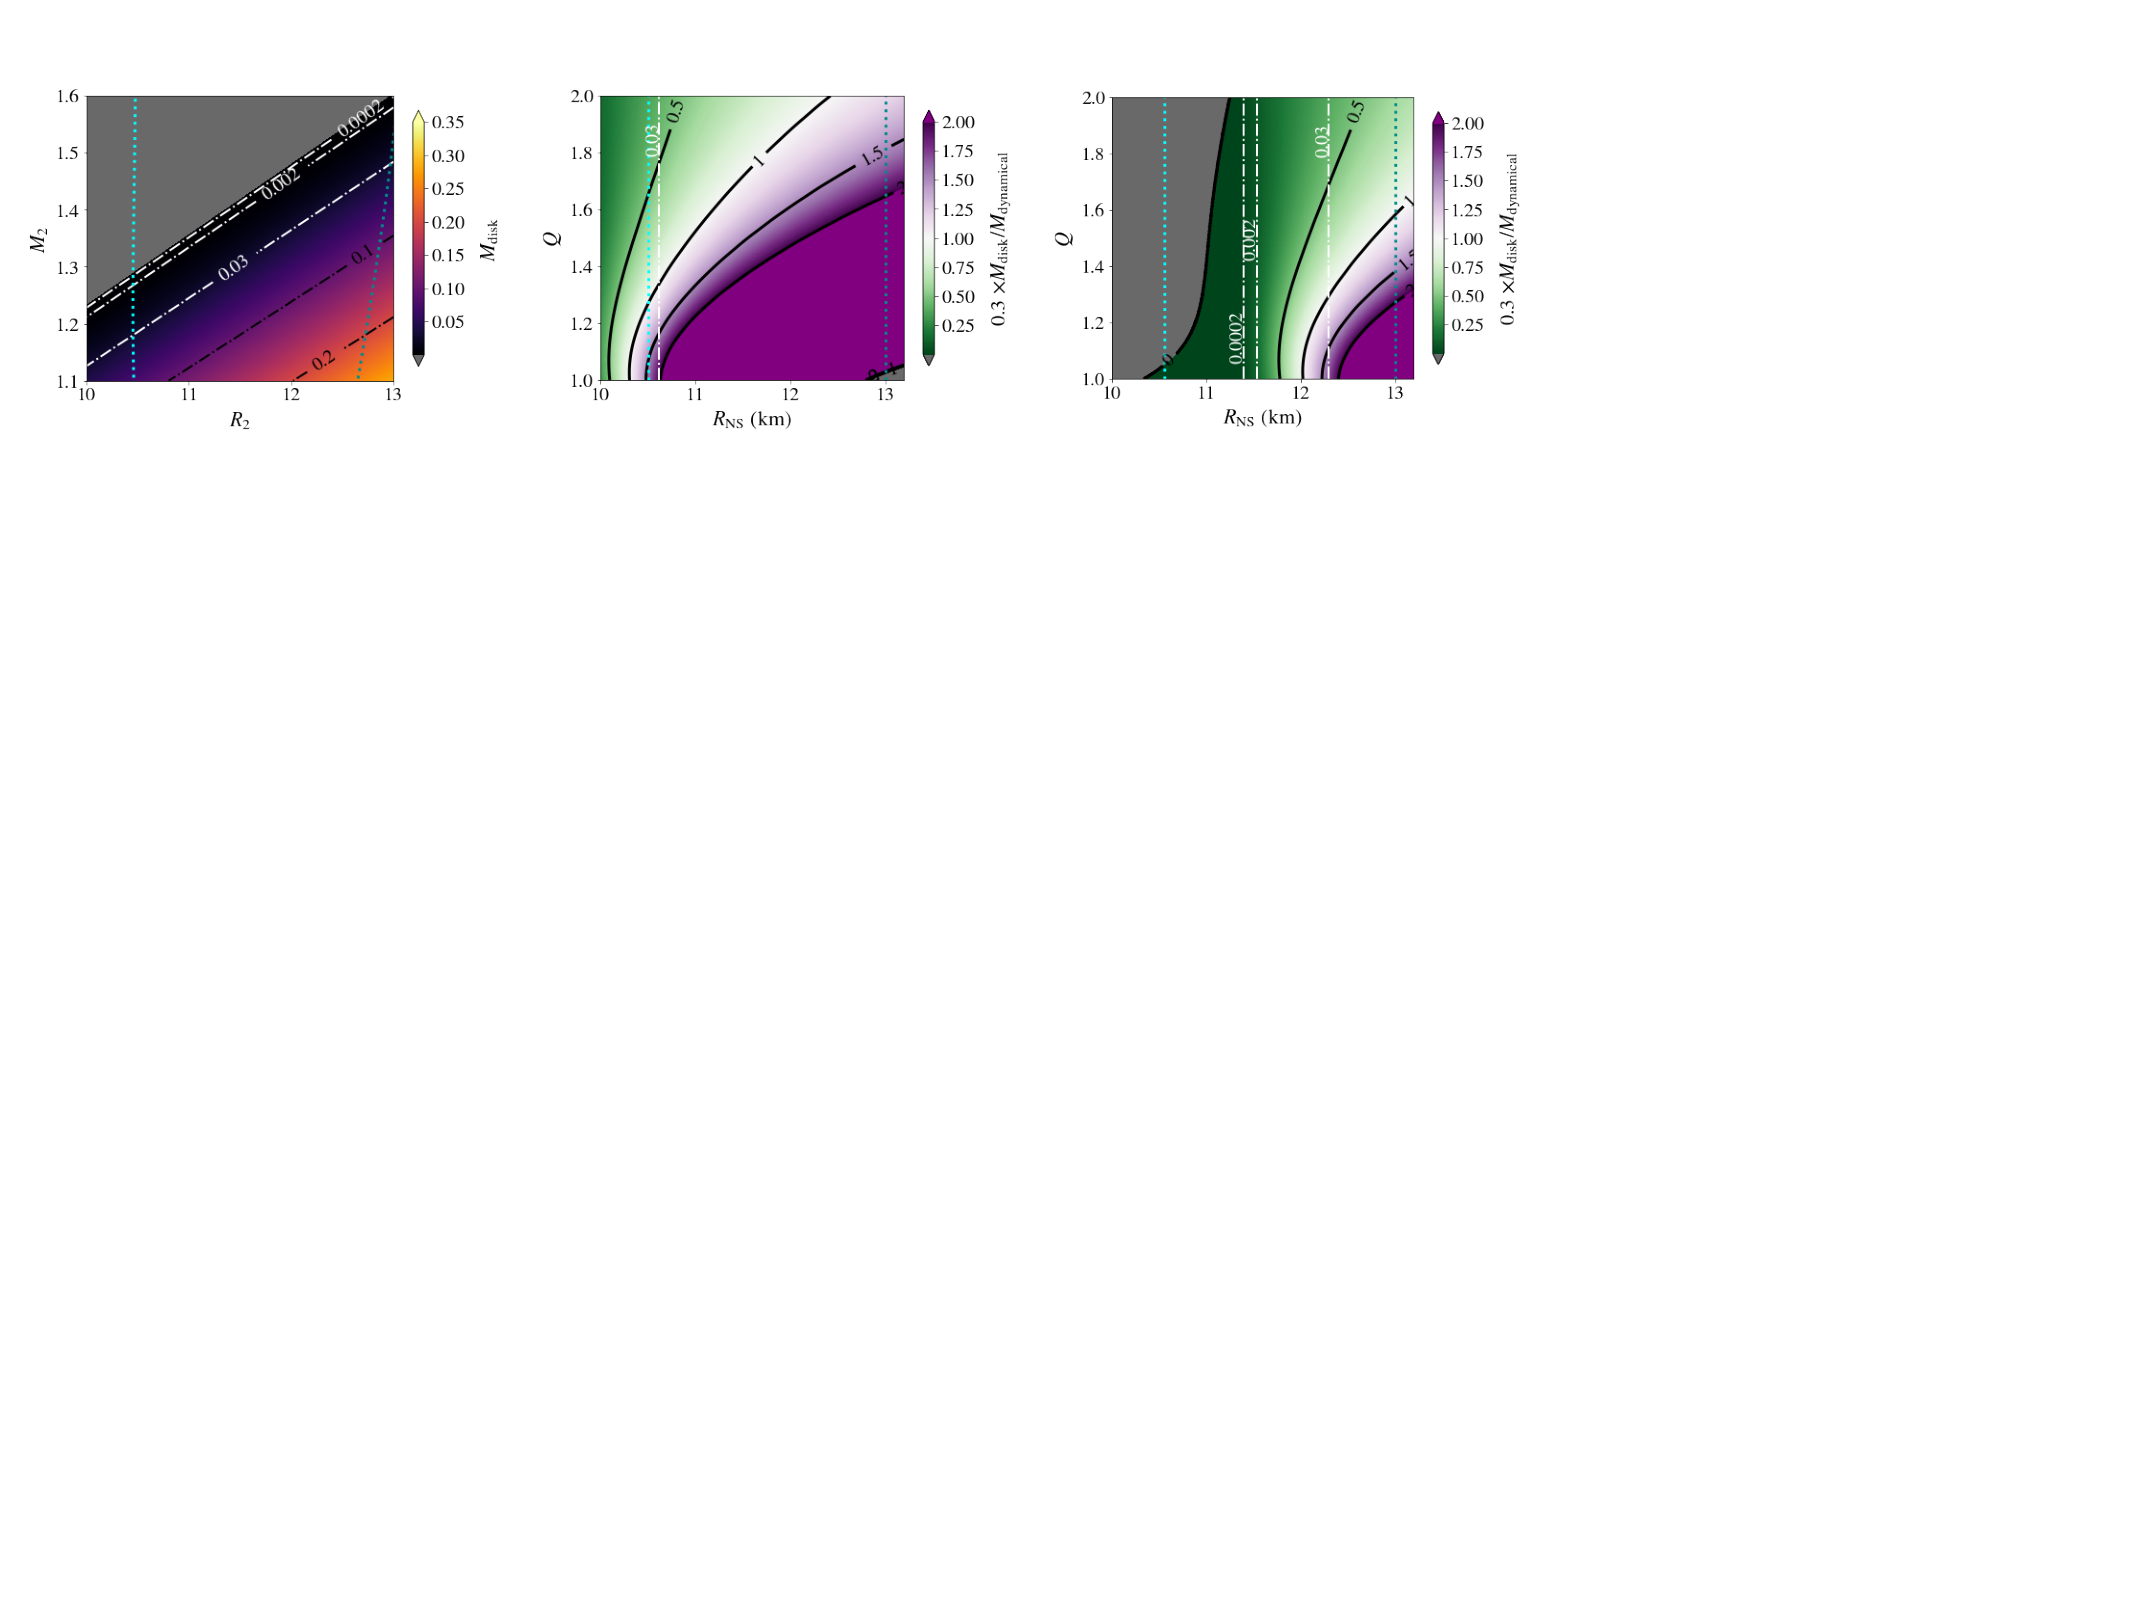
\includegraphics[width=22cm]{figures/kilonova/BNS_parameters_plot.pdf}
\caption{Approximate mapping between binary parameters and accretion disk as well as ejecta masses for binary neutron star systems. Left: Disk mass as a function of mass and radius of the secondary (less-massive) neutron star. Middle: Ratio of disk to dynamical ejecta as a function of the binary mass ratio ($Q = M_1/M_2$) and radius of the component neutron stars (assuming both stars have roughly the same radius), with the mass of the secondary fixed to $M_2 = 1.2~M_\odot$ and assuming disk ejecta to be 30\% of the initial disk mass. Right: Same as the middle panel, but for $M_2 = 1.4~M_\odot$. The dot-dashed lines (in white) delineate the disk masses $M_{\rm disk} = 0.03~M_\odot$, $0.002~M_\odot$, $0.0002~M_\odot$ considered for post-merger simulations in this work. Dotted lines (in cyan) show the lower and upper limits of neutron star radii allowed by recent observations~\cite{De:2018uhw,capano_stringent_2020,Miller:2019cac,Riley:2019yda,Landry:2020vaw}.\label{fig:bns_parameters}}
\vspace{5mm}
\end{figure}
\end{landscape}

\begin{landscape}
\begin{figure*}[t]
  \centering
  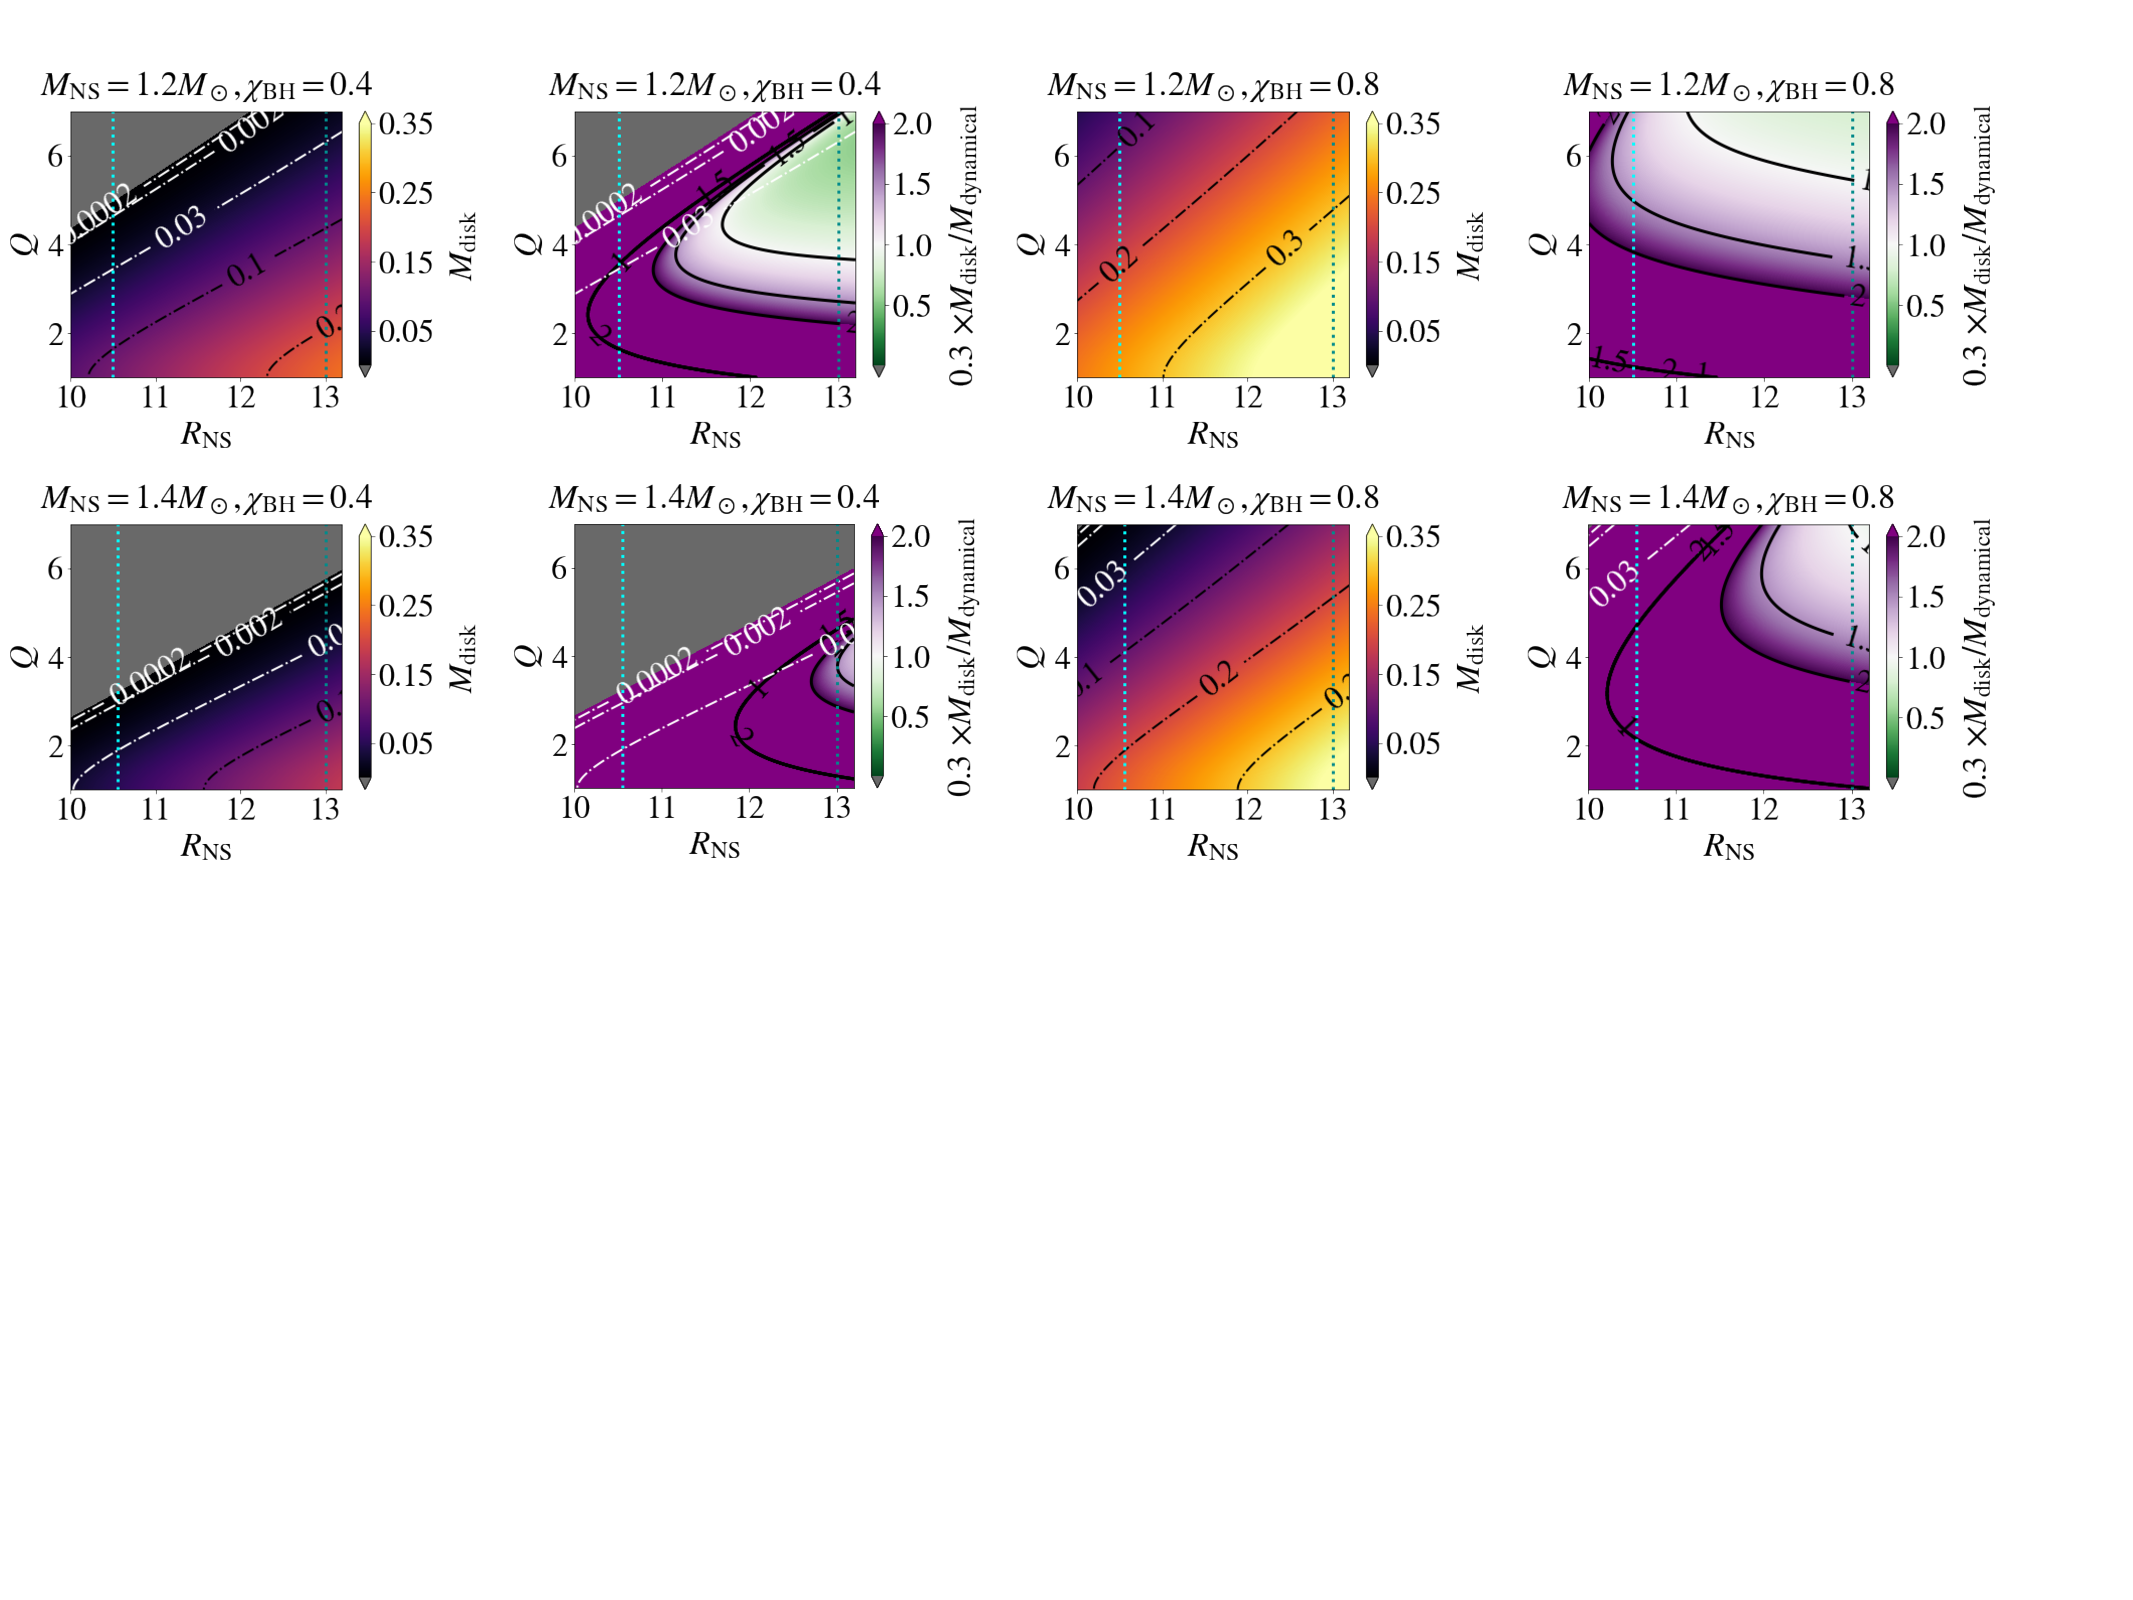
\includegraphics[width=22cm]{figures/kilonova/NSBH_parameters_plot.pdf}
 \caption{Approximate mapping between binary parameters and accretion disk as well as ejecta masses for neutron star-black hole binary systems. Shown are post-merger disk masses and ratios of disk to dynamical ejecta (assuming disk ejecta to be 30\% of the initial disk masses) as a function of the NS radius and the binary mass ratio $Q = M_{\rm BH}/M_{\rm NS}$ for different scenarios, including light and heavier NSs ($M_{\rm NS} = 1.2M_\odot,\, 1.4M_\odot$) and slowly or rapidly spinning BHs (dimensionless spin 0.4 or 0.8). The dot-dashed lines (in white) indicate the disk masses $M_{\rm disk} = 0.03~M_\odot$, $0.002~M_\odot$, $0.0002~M_\odot$ considered for the simulations in this work. Dotted lines (in cyan) show the lower and upper limits of neutron star radii allowed by observations as in Fig.~\ref{fig:bns_parameters}.\label{fig:nsbh_parameters}}
\vspace{5mm}
\end{figure*}
\end{landscape}

Both the binary mass ratio and the EOS determine the dominant source of ejecta in BNS mergers. Disk ejecta dominates across most of the parameter space for small total-mass systems (middle panel of Fig.~\ref{fig:bns_parameters}), except for very small NS radii $\lesssim\!10.5$\,km and large mass ratios $Q\gtrsim 1.6$, while dynamical ejecta dominates in high total-mass systems (right panel of Fig.~\ref{fig:bns_parameters}), unless for larger NS radii $\gtrsim\!12$\,km and small-to-medium mass ratios $Q\lesssim 1.4$. For low-mass BNS systems, the disks simulated here cover the parameter space for small NS radii $\lesssim\!11$\,km, while for high-mass systems they span a wide range of $11\lesssim R_{\rm NS}\lesssim 12.5$\,km. We note that the results of our highest-$M_{\rm disk}$ run can be qualitatively extrapolated to larger disk masses and thus cover most of the remaining parameter space; however, for very massive disks effects of self-irradiation of the outflows become increasingly significant, leading to a more pronounced tail of `blue' ejecta \cite{miller_full_2019-1}. Depending on the secondary mass, the disk outflows of our simulated models may or may not dominate the total ejecta from the system.

In NSBH systems, dynamical ejecta and post-merger accretion disks only arise if the NS is tidally dirupted by the BH. This disruption process requires the tidal disruption radius to reside outside of the innermost stable circular orbit of the BH, and it thus depends on the spin $\chi_{\rm BH}$ of the BH and its mass (and thus on the mass ratio $Q = M_{\rm BH}/M_{\rm NS}$ of the binary). Ouflows from accretion disks typically dominate across most of the parameter space (cf.~Fig.~\ref{fig:nsbh_parameters}, except for light NSs (~$1.2M_\odot$) with large NS radii $\gtrsim 11.5$\,km and medium-to-large mass ratios $Q\gtrsim 3-4$, somewhat dependent on the BH spin.

In the NSBH parameter space, our models simulated here reside in the unequal mass ratio, low BH-spin regimes. Disk ejecta is dominant in this regime, and dynamical ejecta is absent.

%In the NSBH parameter space, our models lie in the unequal mass ratio, low spin regimes. Disk ejecta is dominant in this regime, and dynamical ejecta is absent.

%In the BNS parameter space, our models correspond to low total mass with soft equation of state merger scenarios, or high total mass with stiff equation of state scenarios. \texttt{MD\_M03} covers the regime where disk mass ejecta is dominant or subdominant, whereas \texttt{MD\_M002} and \texttt{MD\_M0002} cover the regime where dynamical ejecta is dominant.



\section{Numerical Methods}
\label{sec:methods}

%comment on grid setup (box sizes, resolution etc.)
\subsection{Simulation setup}\label{subsec:sim_setup}
We perform simulations in ideal GRMHD and full 3D with a fixed background spacetime for computational efficiency using the code and numerical setup described in Ref. \cite{Siegel:2017jug}. The code is based on \texttt{GRHydro}~\cite{mosta_grhydro:_2014} and makes use of the \texttt{Einstein Toolkit}\footnote{\href{http://einsteintoolkit.org}{http://einsteintoolkit.org}} \cite{maria_babiuc-hamilton_einstein_2019,loffler_einstein_2012,Schnetter:2003rb,Goodale:2002a,Thornburg:2003sf}, with neutrino interactions implemented via a leakage scheme based on Refs. \cite{bruenn_stellar_1985} and \cite{ruffert_coalescing_1996}, and follows the implementation of Refs. \cite{galeazzi_implementation_2013} and \cite{radice_dynamical_2016}. Thermodynamic properties of matter are based on the Helmholtz EOS \cite{timmes_accuracy_1999,timmes_accuracy_2000}, and we compute abundances of nuclei at a given density, temperature, and electron fraction $Y_e$, assuming nuclear statistical equilibrium.

The simulations include a Kerr black hole of mass $3.0 M_\odot$ and dimensionless spin $\chi_{\rm BH} = 0.8$, initially surrounded by a torus of constant specific angular momentum, small constant specific entropy of $8~k_{\rm B}$ per baryon, and initial electron fraction $Y_{\rm e} = 0.1$; we refer to Table \ref{tab:ini_config_torus} for a summary of initial torus properties of simulation runs. Run \texttt{MD\_M03} has been discussed before \cite{siegel_three-dimensional_2017,Siegel:2017jug}, and is further elaborated on here by comparing it to the two new runs \texttt{MD\_M002} and \texttt{MD\_M0002}, which represent lighter accretion disks. The BH-disk problem is formulated in Cartesian, horizon-penetrating Kerr-Schild coordinates. The black-hole mass and spin reflect typical NS merger scenarios (see Sec.~\ref{sec:param_space}). The black hole spins in the case of prompt black hole formation from BNS mergers are typically not larger than $\chi_{\rm BH} \approx 0.8$~\cite{kiuchi_longterm_2009,rezzolla_accurate_2010,bernuzzi_mergers_2014,kastaun_black_2013}, and black hole spins in case of delayed black hole formation are $\chi_{\rm BH} \lesssim 0.7$ \cite{sekiguchi_dynamical_2016}. Furthermore, $\chi_{\rm BH} \sim 0.8$ is significant enough to disrupt the NS and lead to a post-merger accretion disk in NSBH mergers across a wide range in mass ratio (\cite{foucart_black-hole-neutron-star_2012}; see the discussion in Sec.~\ref{sec:param_space}). Our initial tori masses are chosen to reflect a mass range covering the ignition threshold for weak interactions in post-merger disks (cf.~Sec.~\ref{sec:intro_ignition_threshold}) and is typical both for BNS and NSBH scenarios (Sec.~\ref{sec:param_space}).

\begin{table*}
\caption{Initial configurations of the accretion disks simulated here. From left to right: black-hole mass and dimensionless spin, disk mass, inner and outer radius of the disk, radius at maximum density, specific entropy, electron fraction, and maximum magnetic-to-fluid pressure ratio.}
\begin{centering}
\begin{tabular}{cccccccccc}
\hline
Run  & $M_{\rm BH}$ & $a_{\rm BH}$ & $M_{\rm d,0}$ & $R_{\rm in,0}$ & $R_{\rm out,0}$  & $R_0$ & $s_0$ & $Y_{\rm e,0}$ & $p_b/p_{\rm f}$\\
& [$M_{\odot}$] & & [$M_{\odot}$] & [$M_{\rm BH}$] & [$M_{\rm BH}$] &  [km] & [$k_B$/b] & & \\
\hline 
MD\_03 & 3 & 0.8 & 0.03 & 4 & 24 & 30 & 8 & 0.1 & $< 5\times 10^{-3}$ \\
MD\_002 & 3 & 0.8 & 0.002 & 7 & 20 & 45.61 & 8 & 0.1 & $< 5\times 10^{-3}$ \\
MD\_0002 & 3 & 0.8 & 0.0002 & 12 & 20 & 66.27 & 8 & 0.1 & $< 5\times 10^{-3}$ \\
\hline 
\end{tabular}
\par\end{centering}
\label{tab:ini_config_torus}
\end{table*}

The tori are initialized with weak poloidal magnetic seed fields, confined to the interior of the tori and defined by the magnetic vector potential $A^r = A^{\theta} = 0$ and $A^{\phi} = A_b$ max$\{p - p_{\rm cut}, 0\}$. Here, $p$ denotes the fluid pressure, $p_{\rm cut}$ is the pressure below which the magnetic field is set to zero, and $A_b$ sets the initial field strength. Here, $p_{\rm cut} \approx 1\times 10^{-2} p_{\rm max}$ in all cases, where $p_{\rm max}$ is the pressure at maximum density in the torus. We choose $p_{\rm cut}$ such that the magnetic field covers the bulk volume of the torus, while preventing it from becoming buoyant in the outermost layers and violently breaking out of the torus at the start of the simulation. We adjust $A_b$ such that the magnetic-to-fluid pressure ratio in the torus is a small value, $p_{\rm B}/p_{\rm f} < 5\times 10^{-3}$.

The initial torus is embedded in a tenuous atmosphere with $T = 10^5$ K, and $Y_{\rm e} = 1$ and $\rho \approx$ 37 g cm$^{-3}$, $\rho \approx$ 3.7 g cm$^{-3}$, and $\rho \approx$ 0.37 g cm$^{-3}$ for runs \texttt{MD\_M03}, \texttt{MD\_M002}, and \texttt{MD\_M0002}, respectively. The density and temperature are chosen such that they are sufficiently low to neither impact the dynamics nor the composition of the disk outflows. The atmosphere densities are set to approximately scale with the maximum density of the accretion disk during the evolution (cf.~Tab.~\ref{tab:torusenergytab}). The total atmosphere mass of the entire computational domain is $3.8\times 10^{-5} M_\odot$ for \texttt{MD\_M03}, $3\times 10^{-7} M_\odot$ for \texttt{MD\_M002}, and $3\times 10^{-8}$ for \texttt{MD\_M0002}, orders of magnitude smaller than the disk ejecta (cf.~Tab.~\ref{tab:torusenergytab}); over a volume of radius 1000\,km, which we consider as the minimum radius for outflow material to be unbound from the BH-disk system, the corresponding atmosphere masses are $1.8\times 10^{-8} M_\odot$ for \texttt{MD\_M03}, $1.8\times 10^{-9} M_\odot$ for \texttt{MD\_M002}, and $1.8\times 10^{-8} M_\odot$ for \texttt{MD\_M0002}). At the chosen atmosphere temperature of $T = 10^5$\,K weak interations are frozen out.

The computational domain represents a Cartesian grid hierarchy centered around the black hole. The grid has eight refinement levels, with an extent in each coordinate direction of $1.53\times 10^4$ km for \texttt{MD\_M03}, and $1.14\times 10^4$ km for \texttt{MD\_M002} and \texttt{MD\_M0002}. The initial tori have diameters of 240~km, 206~km, and 206~km for simulations \texttt{MD\_M03}, \texttt{MD\_M002}, and \texttt{MD\_M0002}, respectively. The initial tori are encompassed by the finest refinement level of the corresponding grid hierarchy. Following previous work \cite{siegel_magnetorotational_2013,Siegel:2017jug,siegel_collapsars_2019}, the finest resolution is $\Delta_{xyz} \approx 850$\,m for all simulations, chosen such that the MRI is well resolved in the stationary turbulent state of the disk (typically by ten grid points per fastest-growing MRI mode), which ensures convergence of global observables (see, e.g., \cite{siegel_collapsars_2019}).

Angular momentum transport is mediated by magnetic turbulence, driven by the MRI, in our setups. The initial tori undergo a relaxation phase with self-consistent magnetic-field amplification, and settle into a quasi-stationary phase at $\sim\!20$ ms. We consider the relaxed state of the disks at this time as the actual initial data for our simulations, and exclude the early transient phase from our analysis---in particular, all material accreted onto the black hole or ejected via outflows during this phase.

\subsection{Diagnostics}\label{subsec:diagnostics}

In order to monitor certain physical quantities in the disk, we compute radial profiles of such a quantity $\chi(\varpi)$ by performing azimuthal, density-weighted averages, integrating up to one scale height of the disk:
%Azimuthal averages of a quantity $\chi$ are defined as
%\begin{equation}
%    \langle \chi \rangle_\phi = \frac{\int^{2\pi}_{0} \chi \sqrt{\gamma_{\phi \phi}}d\phi}{\int^{2\pi}_{0} \sqrt{\gamma_{\phi \phi}}d\phi}
%\end{equation}
%where $\gamma_{ij}$ are the spatial components of the metric tensor $g_{\mu\nu}$ in 3+1-split. We define density-weighted averages 
\begin{equation}\label{eq:radial_av}
    \langle \chi \rangle_{{\rm azim}, z_H} = \frac{\int^{z_H}_{-z_H} \int_0^{2\pi} \chi \hat D \varpi d\phi dz}{\int^{z_H}_{-z_H} \int_0^{2\pi} \hat D \varpi d\phi dz}.
\end{equation}
Here, $\varpi = \sqrt{x^2 + y^2}$ is the cylindrical radius, $\hat D = \sqrt{\gamma} \rho W$ is the conserved rest-mass density as seen by the Eulerian observer moving normal to the spatial hypersurfaces in the 3+1 split of Kerr-Schild spacetime, $\gamma$ is the determinant of the spatial metric $\gamma_{ij}$ in 3+1 split, and $W$ the Lorentz factor of the fluid. The density scale height $z_H$ is defined as
\begin{equation}
    z_H (\varpi) = \frac{\int \int_0^{2\pi} |z| \hat D \varpi d\phi dz}{\int \int_0^{2\pi}\hat D \varpi d\phi dz}.
\end{equation}
By integrating up to the local density scale height, we exclude the disk corona and winds from the calculation. For some quantities, temporal averages $\langle\cdot\rangle_t$ (cf., eg., Eqs.~\eqref{eq:alpha_visc_def_1D} and \eqref{eq:alpha_visc_def_0D}) over a specified time window are taken, in order to reduce the effect of temporal fluctuations of a turbulent medium.

For some disk quantities, it is useful to compute the rest-mass density average and study its evolution over time. We define this averaging as
\begin{equation}\label{eq:rest_mass_dens}
 \langle \chi \rangle_{\hat D} = \frac{\int \chi \hat D d^3x}{\int \hat D d^3x}.
\end{equation}
In some cases, this average is calculated by integrating only up to the local scale height,
\begin{equation}\label{eq:rest_mass_dens_scaleht}
    \langle \chi \rangle_{\hat D, z_H} = \frac{\int^{z_H}_{-z_H} \chi \hat D \varpi dz}{\int^{z_H}_{-z_H} \hat D \varpi dz},
\end{equation}
which allows us to explicitly exclude the disk corona and disk wind regions.


\section{Numerical Results}
\label{sec:results}

We proceed by first discussing our results for global disk properties, such as MHD mediated angular momentum transport (Sec.~\ref{sec:viscosity}), accretion (Sec.~\ref{sec:accretion}), neutrino emission (Sec.~\ref{sec:neutrino_emission}), disk ejecta (Sec.~\ref{sec:ejecta}), before discussing disk evolution locally in terms of weak interactions (Sec.~\ref{sec:disk_composition}) and nucleosynthesis from the disk outflows (Sec.~\ref{sec:nucleosynthesis}).


\subsection{Global properties}
\label{sec:global_properties}

\begin{table*}
\caption{Various properties of the accretion disks simulated here. From left to right: average density, and accretion rate after relaxation, estimated total unbound disk outflow mass ($M_{\rm ej}$; `ejecta') in solar masses and in units of the total disk mass ($M_{\rm tot}$) after relaxation, with mean electron fraction, initial total neutrino luminosity in electron and anti-electron neutrinos, effective $\alpha$-viscosity parameter, viscous evolution time and total evolution time for the respective runs. The averages $\bar{\rho}_{\rm d}$ and $\bar \alpha_\mathrm{vis}$ with the quoted uncertainties represent density-weighted average, maximum, and minimum values around a 10\,ms window centered at $t = 30$\,ms (see the text for details). The values for $\dot{M}_{d}$ with quoted uncertainties represent the average, maximum, and minimum values over the same time window at $t = 30$\,ms. The values for $L_{\nu,\mathrm{max}}$ represent the average value extracted from the neutrino luminosity over a 10\,ms window centered at the global peak luminosity of anti-electron neutrinos.
}
\setlength{\tabcolsep}{5pt}
\begin{centering}
\begin{adjustwidth}{-1.25cm}{}
{\normalsize\renewcommand{\arraystretch}{.8}
\resizebox{!}{.045\paperheight}{%
\begin{tabular}{cccccccccc}
\hline
Run  & $\bar{\rho}_{\rm d}$ & $\dot{M}_{d}$  & $M_{\rm ej}$ & $M_{\rm ej}/M_{\rm tot}$ & $\bar{Y}_e$ & $L_{\nu,\mathrm{max}}$ & $\bar \alpha_\mathrm{vis}$ & $t_{\rm visc}$ & $t_{\rm end}$\\
 & [$\mathrm{g}\,\mathrm{cm}^{-3}$] & [$M_{\odot}\,\mathrm{s}^{-1}$] &  [$M_{\odot}$] & & & [$\mathrm{erg}\,\mathrm{s}^{-1}$] & & [ms] & [ms]\\
\hline 
MD\_03 & $5.53_{-1.4}^{+2.2}\times 10^{10}$ & $2.6_{-0.7}^{+1.4}\times 10^{-1}$ & $3.179\times 10^{-3}$ & 0.157 & 0.174 & 2.1$\times 10^{52}$ & $1.76_{-1.7}^{+2.8}\times 10^{-2}$ & 279 & 381\\
MD\_002 & $6.6^{+0.5}_{-0.9}\times 10^9$ & $1.14_{-0.4}^{+0.4}\times 10^{-2}$ & $4.030\times 10^{-4}$ & 0.171 & 0.114 & 14$\times 10^{50}$ & $1.01_{-0.6}^{+1.5}\times 10^{-2}$ & 874 & 309\\
MD\_0002 & $3.4^{+0.7}_{-0.6}\times 10^8$ & $3.79_{-1.7}^{+2.5}\times 10^{-4}$ & $6.046\times 10^{-5}$ & 0.356 & 0.101 & 2.1$\times 10^{48}$ & $1.14_{-1.1}^{+2.0}\times 10^{-2}$ & 1731 & 294\\
\hline 
\end{tabular}
}}
\end{adjustwidth}
\par\end{centering}
\label{tab:torusenergytab}
\end{table*}

\subsubsection{MHD turbulence \& effective viscosity}
\label{sec:viscosity}

%\textcolor{red}{note that amplification of B-filed and development of MHD turbulence self-consistent from much weaker fields as in previous papers. Discuss computation of effective alpha-viscosity parameter and include \& describe plot (similar as in collapsar paper). Remark that it's a constant among the simulations and in above equation, hence the scaling between Mdot and rho\_d.}

\begin{figure}[t]
\centering
  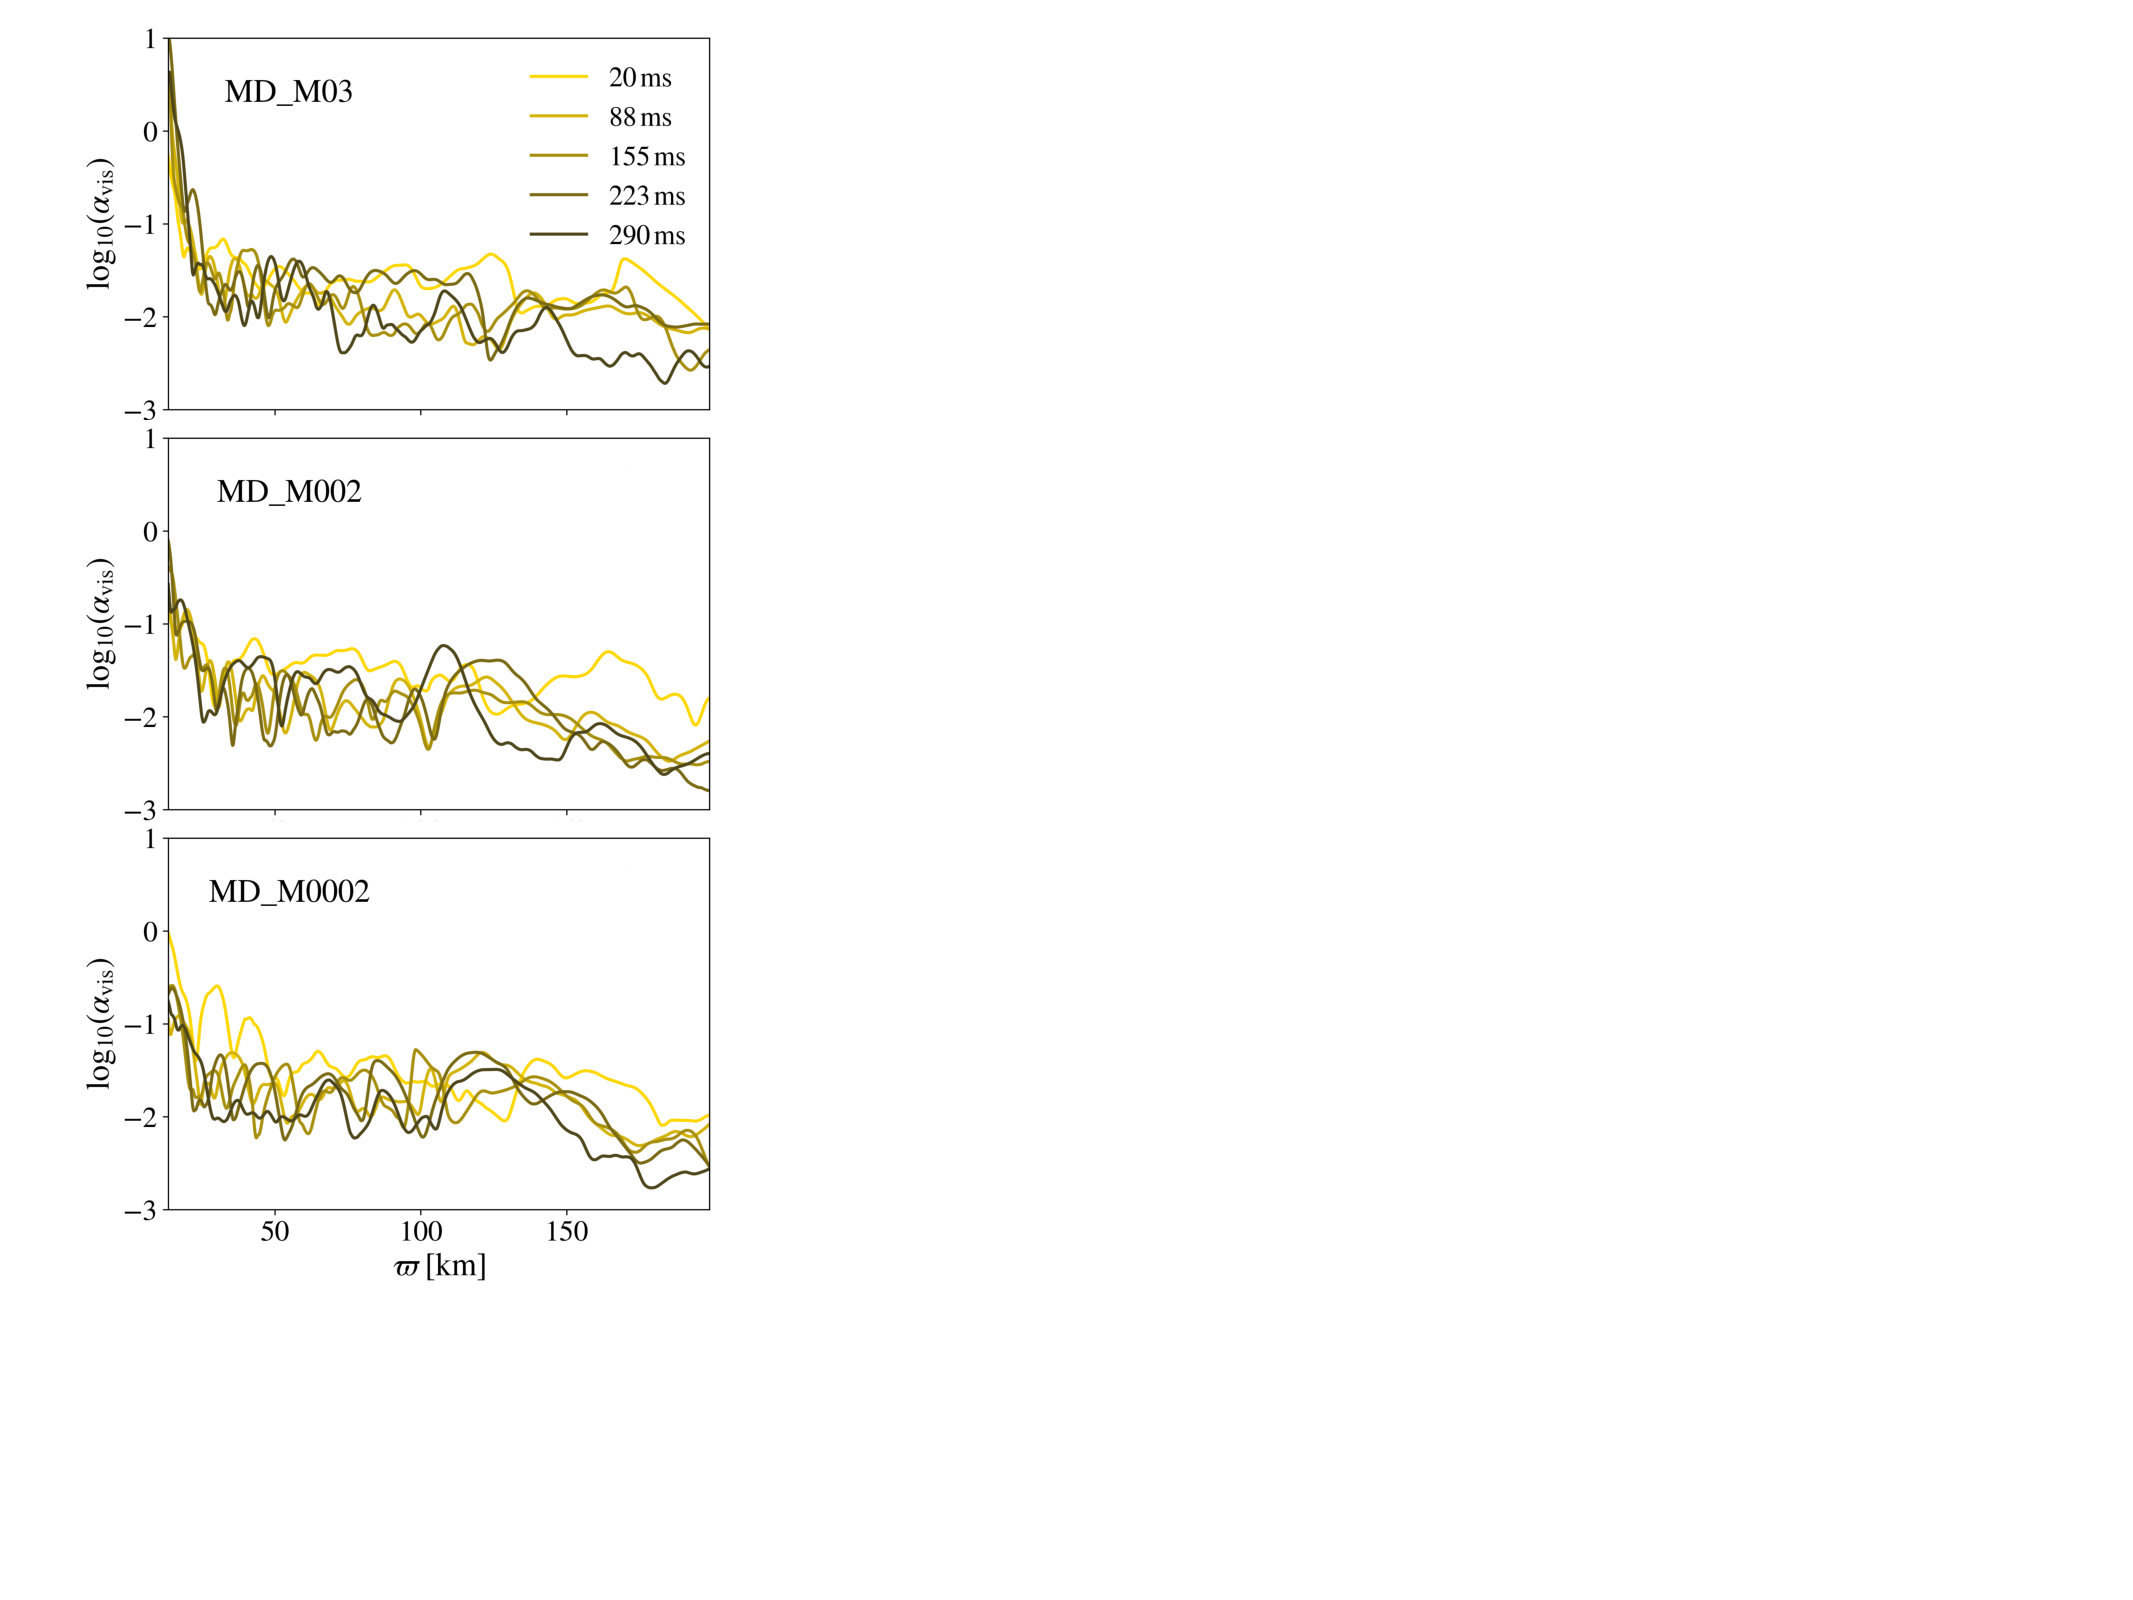
\includegraphics[width=10cm]{figures/kilonova/alpha-viscosity.pdf}
 \caption{Radial profiles of the effective Shakura-Sunyaev viscosity parameter $\alpha_{\rm vis}$ defined in Eq.~\eqref{eq:alpha_visc_def_0D} at different times during the evolution for the three simulation runs in this work. \label{fig:alpha-viscosity}}
\vspace{5mm}
\end{figure}

Soon after the start of the simulations, our accretion disks show vigorous magnetic turbulence, triggered by the MRI, a local fluid instability developed in differentially rotating magnetized fluids~\cite{velikhov_notitle_1959,chandrasekhar_stability_1960,balbus_powerful_1991,balbus_instability_1998,balbus_enhanced_2003,armitage_dynamics_2011}. The initial weak magnetic field in the simulations is purely poloidal, and it is amplified by the MRI at an exponential rate. As the simulation progresses, a toroidal field component is initially amplified by magnetic winding, before the toroidal field becomes susceptible to the MRI as well. This combination of the MRI and magnetic winding causes an overall increase of the maximum total magnetic field strength. At $t\approx 20$~ms, a steady turbulent state is achieved by the disk and the magnetic field, self-consistently amplified by the MRI, reaches saturation, loosing memory of the initial magnetic field configuration. We refer to Ref. \cite{siegel_three-dimensional_2018} for a more detailed discussion on how this turbulent state arises.

MHD turbulence in the disk operates as large-scale viscosity, which can be parameterized by an effective Shakura-Sunyaev viscosity $\alpha_{\rm vis}$. We define this quantity as
\begin{equation}
    \alpha_{\rm vis} (\varpi) = \frac{\langle \langle |T^{r,\phi}|\rangle_{{\rm azim}, z_H}\rangle_t}{\langle \langle p \rangle_{{\rm azim}, z_H}\rangle_t}, \label{eq:alpha_visc_def_0D}
\end{equation}
where $T^{r,\phi}$ is the $r-\phi$ component of the stress-energy tensor in the frame comoving with the fluid, and $p$ the fluid pressure. Here, time averages are taken over a few neighboring data snapshots.

Figure \ref{fig:alpha-viscosity} shows radial profiles of $\alpha_{\rm vis}$, computed using Eq.~\eqref{eq:radial_av}, at different times during the disks' evolution, for all three simulation runs. We find that $\alpha_{\rm vis}$ is roughly constant among the simulations, independent of the initial disk mass. Table \ref{tab:torusenergytab} reports global values for $\alpha_{\rm vis}$ for each simulation. The latter values describe the accretion state of the inner disk. We compute these values as an average over a 10~ms time-window centered at $t = 30$~ms, extracted from the time evolution of the absolute value of the rest-mass density average of $\alpha_{\rm vis}$,
\begin{equation}
    \alpha_{\rm vis} = \frac{\langle \langle |T^{r,\phi}|\rangle_{\hat{D}, z_H}\rangle_t}{\langle \langle p \rangle_{\hat{D}, z_H}\rangle_t}. \label{eq:alpha_visc_def_1D}
\end{equation}
The rest-mass density average is calculated following the procedure in Equation \eqref{eq:rest_mass_dens_scaleht}, restricting to the region between 30-175\,km from the centers of the black holes. By applying this restriction along the radial extent, only the inner disk regions that can be directly related to the accretion rate onto the black hole are used in the calculation; the data of the outer parts of the disks that start to viscously spread are excluded from the calculation. Also excluded are the innermost regions that show a rise of $\alpha_\mathrm{eff}(\varpi)$ toward the innermost stable circular orbit and the black-hole horizon due to increasing mean magnetic field strengths (\cite{penna_shakura-sunyaev_2013}; cf.~Fig.~\ref{fig:alpha-viscosity}). As indicated by the radial profiles in Fig.~\ref{fig:alpha-viscosity}, the averages for $\alpha_{\rm vis}$ in the inner disks as reported in Tab.~\ref{tab:torusenergytab} are roughly constant among the different accretion disks explored here.

The extraction of effective $\alpha$-viscosities allows us to compute approximate viscous evolution timescales for our disks,
\begin{eqnarray}
	t_{\rm visc} &=& \frac{1}{\alpha}\left(\frac{R_0^{3}}{GM_{\rm BH}}\right)^{1/2}\left(\frac{z_H}{\varpi}\right)^{-2} \label{eq:tvisc} \\
	\approx&& \mskip-15mu 2.6\,{\rm s} \left( \frac{\alpha}{0.01}\right)^{-1}\mskip-5mu\left(\frac{R_0}{30\,{\rm km}}\right)^{\frac{3}{2}} \mskip-5mu\left(\frac{M_{\rm BH}}{3M_\odot}\right)^{-\frac{1}{2}} \mskip-5mu\left(\frac{z_H/\varpi}{0.1}\right)^{-2}\mskip-5mu, \nonumber
\end{eqnarray}
where we have normalized to typical values in our context in the second line. For further reference, viscous timescales for our simulation runs are listed in Tab.~\ref{tab:torusenergytab}. For all disks we find that the effective viscous timescales are typically of the order of a few seconds, and thus sufficiently long to explain the prompt emission of short gamma-ray bursts with typical durations of $T_{90}<2\,{\rm s}$ via accretion onto a black hole.

%This indicates that for a given $A(r)$, $M_{\rm BH}$, $H$, $r$, the scaling of $\dot M$ with $\bar{\rho}_{\rm d}$ always is a constant. $\dot M$ in the simulations is self-consistently set by MHD turbulence to obey this relation.




\subsubsection{Accretion}
\label{sec:accretion}

\begin{figure}[t]
  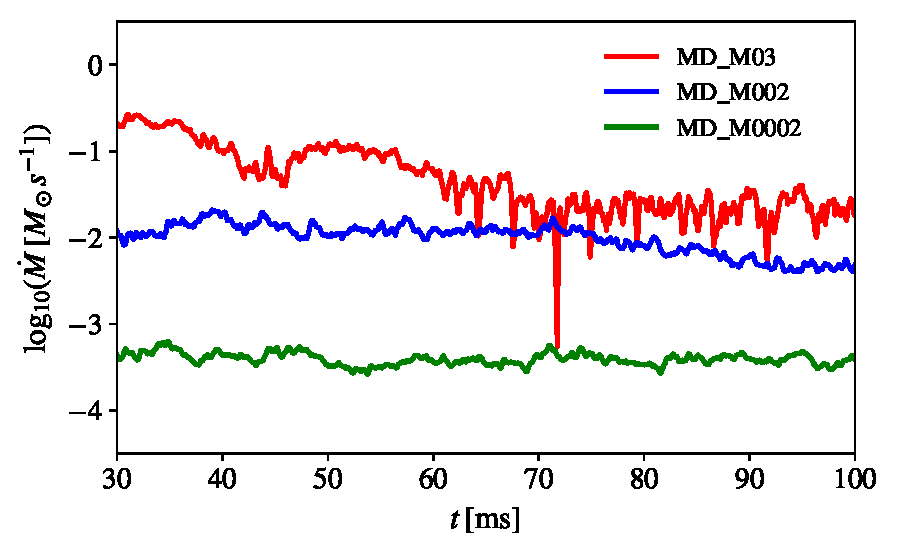
\includegraphics[width=\columnwidth]{figures/kilonova/Mdot_acc_multidets_sims.pdf}
  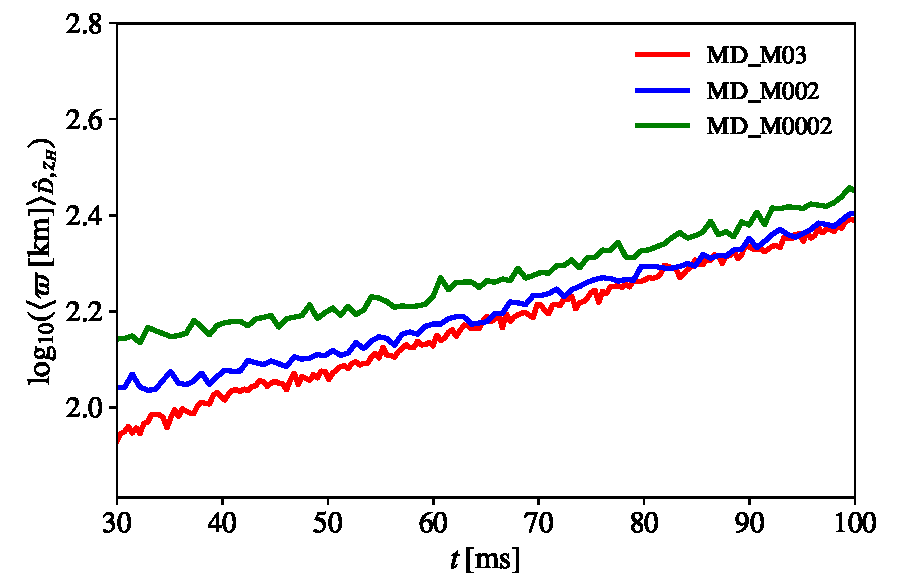
\includegraphics[width=\columnwidth]{figures/kilonova/mean_radius_multi_densav_log.pdf}
 \caption{Top: Black hole accretion rates as a function of time for the three simulation runs in this work. Bottom: Density-averaged cylindrical radius of matter as a function of time, indicating viscous spreading over time. \label{fig:mdot-t}}
%\vspace{5mm}
\end{figure}

\begin{figure}[t]
  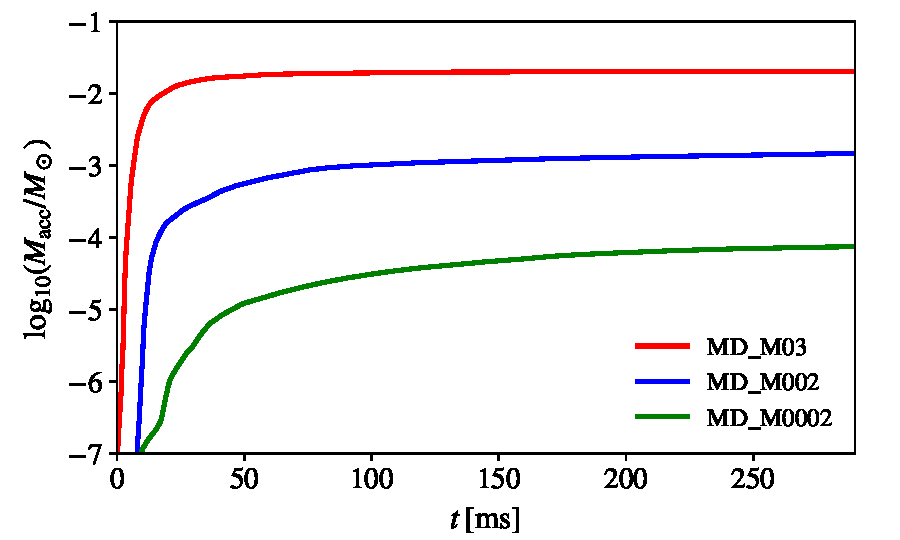
\includegraphics[width=\columnwidth]{figures/kilonova/Macc_multidets_sims.pdf}
 \caption{Top: Black hole accretion rate as a function of time for the three simulation runs in this work. As a result of viscous spreading, the total cumulative accreted mass essentially converges over the duration of the simulation runs, and all remaining material will be eventually unbound from the system. \label{fig:macc-t}}
%\vspace{5mm}
\end{figure}

Magnetic turbulence in the disks generated by the MRI drives accretion onto the black hole at the center, and outward transport of angular momentum in the disks. Figure \ref{fig:mdot-t} shows the evolution of accretion rates $\dot M$ with time for all three simulations. The accretion rates for models \texttt{MD\_M03}, \texttt{MD\_M002}, and \texttt{MD\_M0002}, time-averaged over a 10\,ms window around $t=30$\,ms are $2.6_{-0.7}^{+1.4}\times 10^{-1}~M_\odot s^{-1}$, 
$1.14_{-0.4}^{+0.4}\times 10^{-2}~M_\odot s^{-1}$, and $3.79_{-1.7}^{+2.5}\times 10^{-4}~M_\odot s^{-1}$ respectively; the accretion rate changes by a similar order of magnitude as the disk masses among the three simulation runs, which is expected from one-dimensional disk models.

From one-dimensional disk models (see Appendix \ref{app:ignition_threshold}, Eq.~\eqref{eq:Mdot_1D_2}),
\begin{equation}
    \dot{M} \propto \alpha_{\rm vis} \bar{\rho}_{\rm d} M_{\rm BH}^{1/2} \left(\frac{z_H}{\varpi}\right)^3, \label{eq:Mdot}
\end{equation}
where $\bar{\rho}_{\rm d}$ is the disk density. We compute a representative value for $\bar{\rho}_{\rm d}$ in the inner accretion disk by calculating a three-dimensional spatial average of the disk following Eq.~\eqref{eq:rest_mass_dens_scaleht}, time-averaged over a 10\,ms window around $t=30$\,ms (see Tab.~\ref{tab:torusenergytab}). We note that the quantities, self-consistently set by MHD turbulence in our simulations, roughly satisfy relation \eqref{eq:Mdot}, within the uncertainties in extracting these numbers given the 3D turbulent evolution of the disks.

The bottom panel of Fig.~\ref{fig:mdot-t} shows the early evolution of the density-averaged cylindrical radius of matter $\langle \varpi \rangle_{{\rm azim}, z_H}$ in the simulations, integrated up to the local density scale height. This parameter is roughly representative of viscous radial spreading of the disks. The early evolution shown in Fig.~\ref{fig:mdot-t} is indeed indicative of viscous spreading of our disks.

As measured by the mass flux through a spherical coordinate detector surface placed at a radius of 12~km, the percent initial disk mass accreted by the black hole is $\approx$ 47\%, $\approx$ 60\%, and $\approx$ 31\% for \texttt{MD\_M03}, \texttt{MD\_M002}, and \texttt{MD\_M0002} respectively, by the end of the simulations. Figure \ref{fig:macc-t} shows the evolution of the accreted mass by the black hole over the duration of the simulations. Most of the accretion completes within the first $\sim$ 50-100~ms, after which the accretion rate starts to drop rapidly, with a comparatively negligible amount of mass projected to be accreted onto the black hole past the end of the simulation. We ascribe this effect to viscous spreading of the disks, which forces the disk material remaining at the end of the simulations to eventually be unbound from the system in the form of winds. Properties of ejecta are discussed in Sec.~\ref{sec:ejecta}.

%$z_H$ of the disk, defined as (cf. Equations 62 and 63 of \citet{Siegel:2017jug})
%\begin{equation}
%    z_H (\varpi) = \frac{\int \int_0^{2\pi} |z|\hat D \varpi d\phi dz}{\int \int_0^{2\pi} \hat D \varpi d\phi dz},
%\end{equation}
%where $\hat D = \sqrt{\gamma} \rho W$ is the conserved rest mass density, with $\gamma$ being the determinant of the spatial metric
%$\gamma_{ij}$ and $W$ the Lorentz factor. In this way, we explicitly exclude the disk corona and winds from the integration.


\subsubsection{Neutrino emission}
\label{sec:neutrino_emission}

\begin{figure*}[t]
  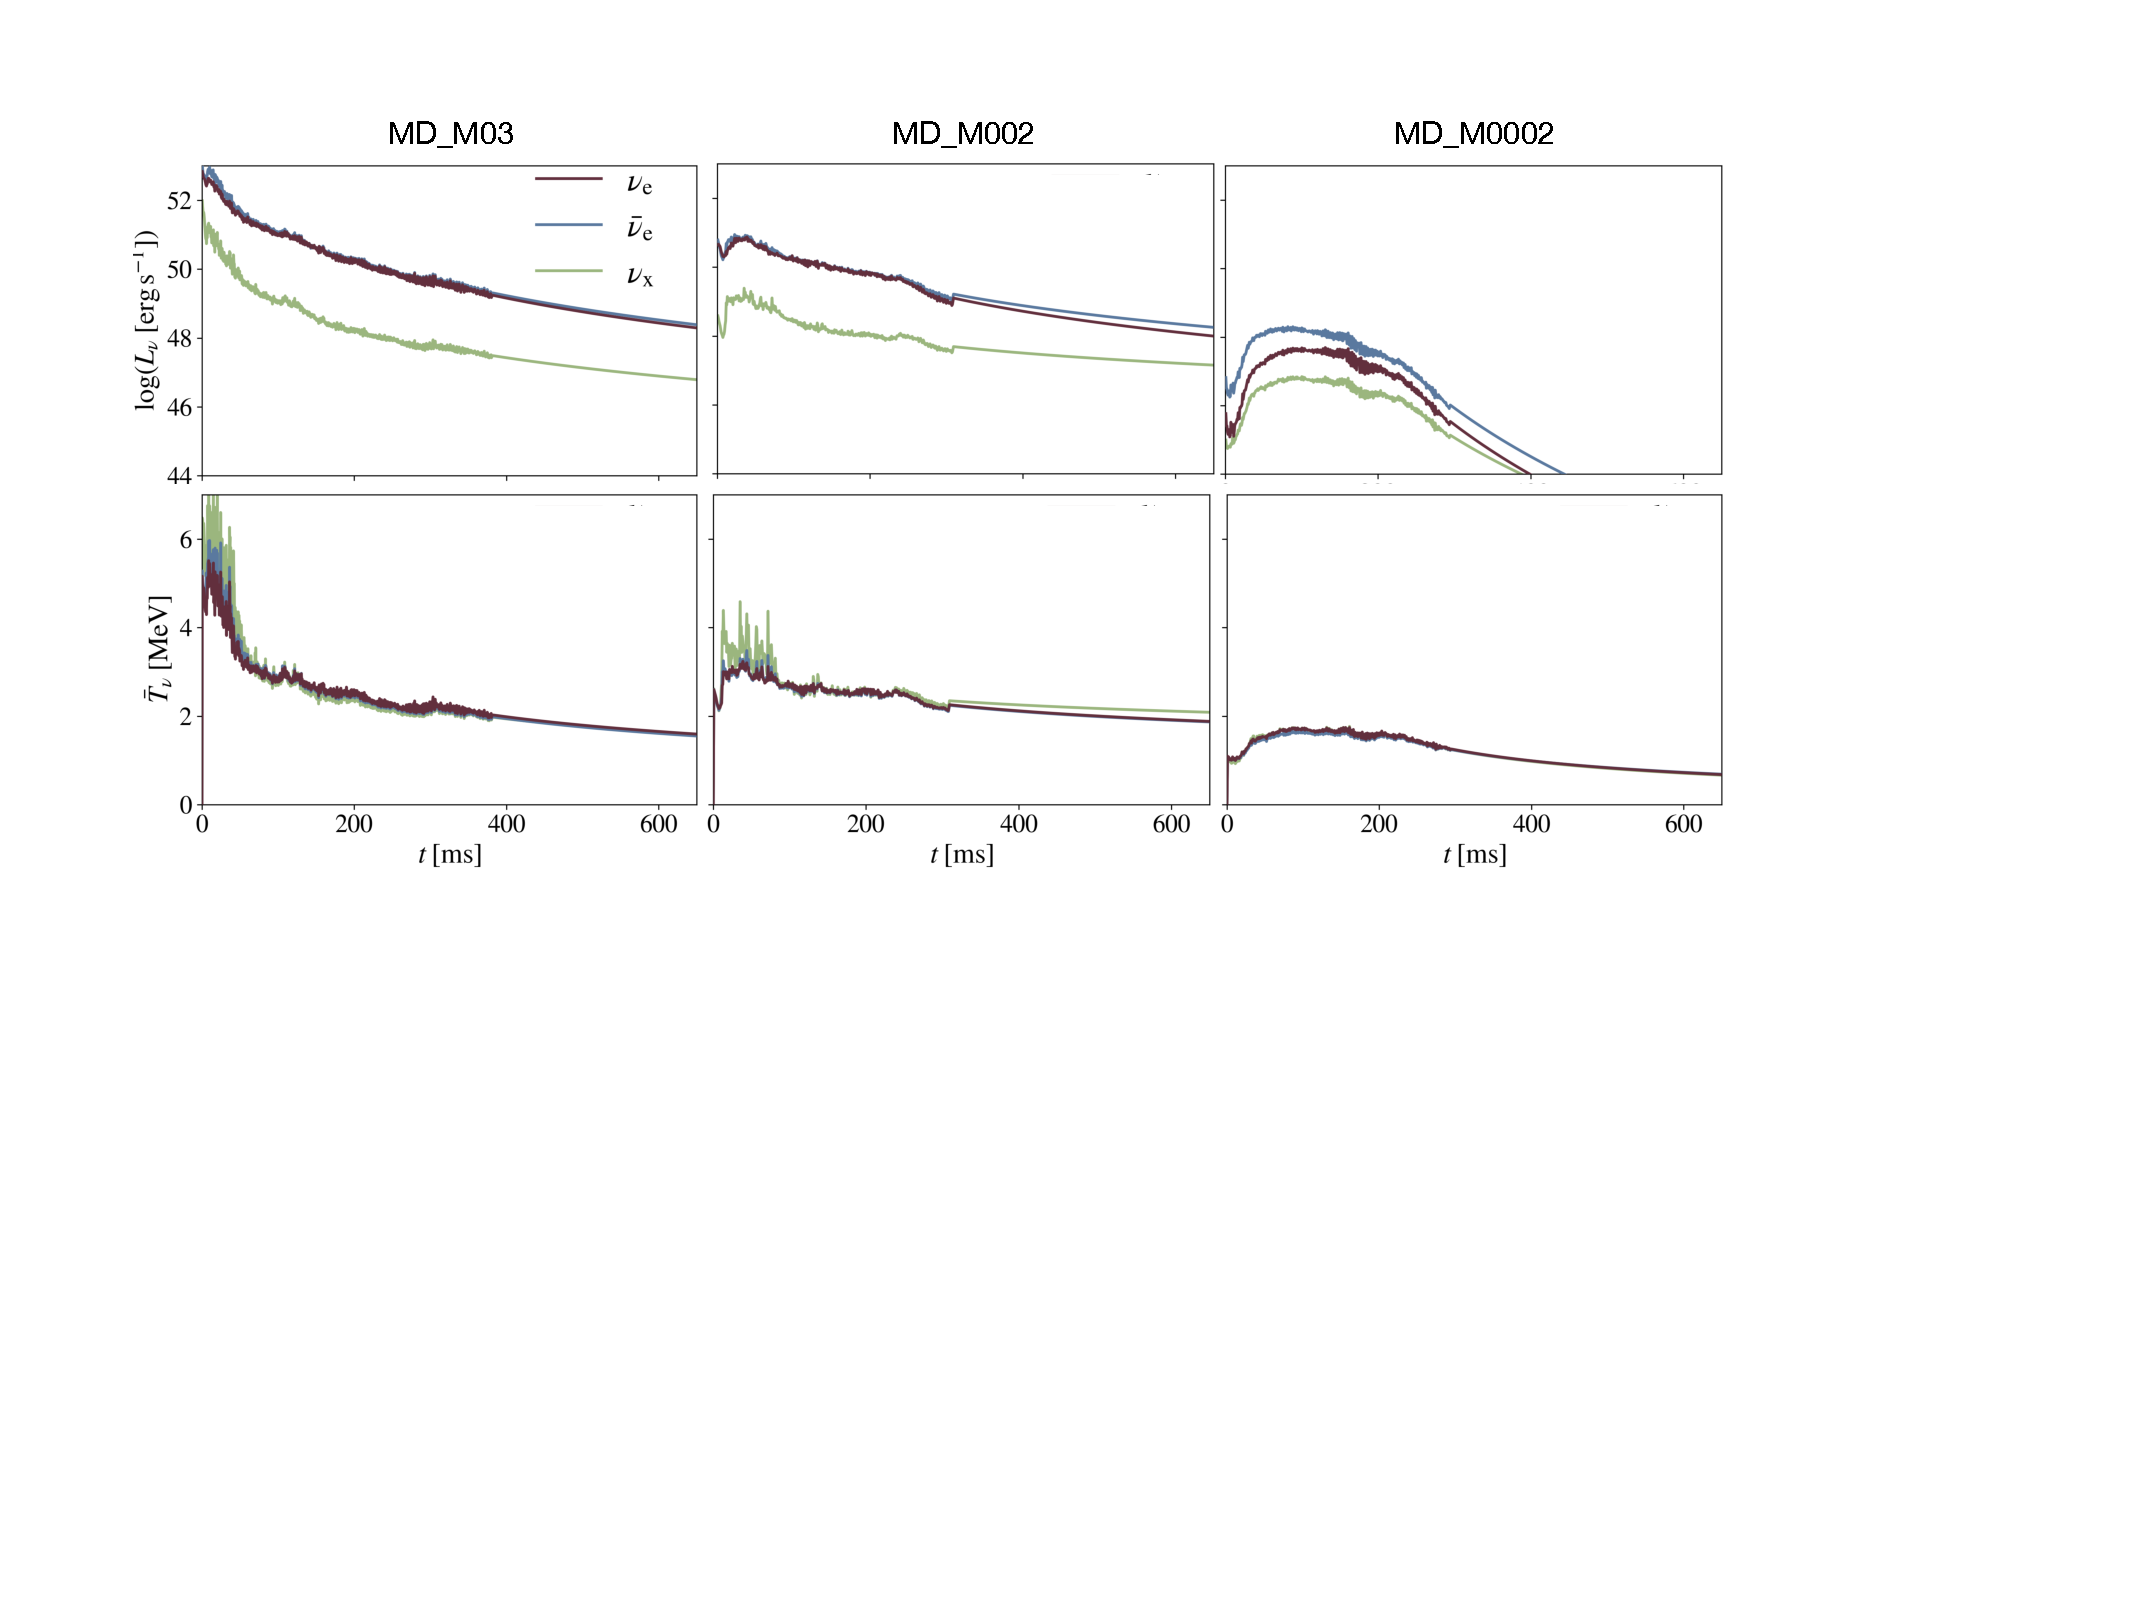
\includegraphics[width=\textwidth]{figures/kilonova/Lum_temp_nu_plots.pdf}
 \caption{Characteristics of neutrino emission from the disk models in this work. The top panels show total neutrino luminosity and the bottom panels show mean neutrino emission temperature. The simulations end at $t \sim\!290$~ms after which the quantities are extrapolated by power law fits to late times.\label{fig:Lum_temp_nu}}
%\vspace{5mm}
\end{figure*}

\begin{figure}[t]
  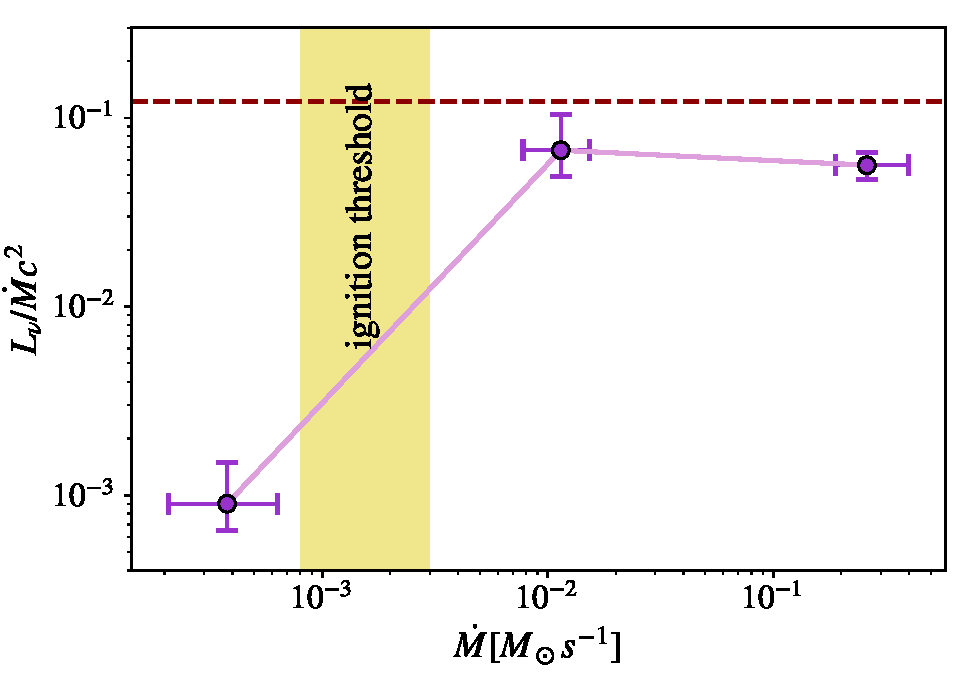
\includegraphics[width=\columnwidth]{figures/kilonova/lum_mdot.pdf}
 \caption{Radiative efficiency as a function of accretion rate for accretion on to a black hole with mass $3~M_\odot$ and dimensionless spin 0.8, as derived from the simulations in this work. The efficiency rises with increasing $\dot M$, reaches a maximum just above the ignition threshold $\dot{M}_{\rm ign}\sim 1\times 10^{-3}\,M_\odot\,{\rm s}^{-1}$ (cf.~Eq.~\eqref{eq:Mdot_ign_merger}), then decreases with increasing $\dot M$. The black dashed line shows the maximum radiative efficiency possible in such a system (see the text for details).\label{fig:lum-mdot}}
%\vspace{5mm}
\end{figure}

Figure \ref{fig:Lum_temp_nu} shows properties of neutrino radiation from the disks for all neutrino species $\nu_i \in {\nu_{e}, \bar \nu_{e}, \nu_{x}}$, where $\nu_{x}$ represents all heavier neutrino species collectively. As in Ref. \cite{Siegel:2017jug}, we define the total neutrino luminosity $L_\nu$ of a given species and the corresponding mean neutrino emission temperature $\bar T_\nu$ as
\begin{equation}
    L_{\nu_i} = \int \alpha W Q_{\nu_i}^{\rm eff} \alpha\sqrt{\gamma}d^{3}x,
\end{equation}
and
\begin{equation}
    \bar T_{\nu_i} = \frac{\int TQ_{\nu_i}^{\rm eff}W\alpha\sqrt{\gamma}d^{3}x}{\int Q_{\nu_i}^{\rm eff}W\alpha\sqrt{\gamma}d^{3}x},
\end{equation}
respectively. Here, $Q_{\nu_i}^{\rm eff}$ is the effective neutrino emissivity, $W$ is the Lorentz factor, and $\alpha$ is the lapse function. We fit power laws to the late time simulation data to extrapolate these quantities beyond the time range modeled in the simulations. Figure \ref{fig:Lum_temp_nu} shows that the electron and anti-electron neutrino luminosities are at least an order of magnitude higher than the heavier neutrino luminosities. Emission channels for the heavier species are relatively suppressed at the comparatively low densities and temperatures of such accretion disks. Luminosities are typically maximal initially when the turbulent state has been established and the disks are still compact and in their high-density and high-temperature regime. Table \ref{tab:torusenergytab} reports the total $L_\nu$-value for $\nu_e$ and $\bar{\nu}_e$ for each simulation run, extracted as an average over a $10$\,ms time-window around the peak luminosties of the respective runs. These range between $\approx\!1\times 10^{52}$\,erg\,s$^{-1}$ (\texttt{MD\_M03}) and $\approx\!1\times 10^{48}$\,erg\,s$^{-1}$ (\texttt{MD\_M0002}). %Table \ref{tab:torusenergytab} reports the initial total $L_\nu$-value for $\nu_e$ and $\bar{\nu}_e$ for each simulation run, extracted as an average over a $10$\,ms time-window centered at the simulation time $t = 30$\,ms, which range between $\approx\!1\times 10^{52}$\,erg\,s$^{-1}$ (\texttt{MD\_M03}) and $\approx\!1\times 10^{48}$\,erg\,s$^{-1}$ (\texttt{MD\_M0002}). 
At later simulation times, as the accretion disks spread radially and become less compact, luminosities start to quickly fade over the timescales of the simulations. This indicates the neutrino self-irradiation of outflows in the context of r-process nucleosynthesis (see Sec.~\ref{sec:nucleosynthesis}) is likely only important initially, and much less so for the less luminous disks \texttt{MD\_M002} and \texttt{MD\_M0002}.
%for \texttt{MD\_M03} and \texttt{MD\_M002}, irradiation by neutrinos in the early part of the disk evolution can have an appreciable effect on the outflows and $r$-process nucleosynthesis. For \texttt{MD\_M0002}, neutrino irradiation is not strong enough to modify the composition of outflows.



The qualitatively different behavior of our disk models in terms of weak interactions is captured by the differences in radiative efficiency $L_\nu/\dot M c^2$ among the simulations. Figure \ref{fig:lum-mdot} shows the variation of the radiative efficiency of the disks as a function of their accretion rate $\dot M$. The ratio $L_\nu/\dot M c^2$ represents the amount of accreted rest-mass energy that is turned into radiation per unit time. In order to assess radiative efficiency, for each simulation, we extract $L_\nu$ and $\dot M$ as mean values over the time range $t = 25-35$~ms. Fig.~\ref{fig:lum-mdot} shows the resulting efficiencies of $5.61^{+0.9}_{-0.9}\times 10^{-2}$, $6.73^{+3.7}_{-1.8}\times 10^{-2}$, and $9.01^{+6.0}_{-2.5}\times 10^{-4}$ for \texttt{MD\_M03}, \texttt{MD\_M002}, and \texttt{MD\_M0002}, respectively, compared to the maximum possible radiative efficiency. The latter is a fundamental limit on the amount of energy that can be extracted from a black hole accretion flow, determined by the available binding energy \cite{thorne_disk-accretion_1974}, 
\begin{equation}
    [L_\nu/\dot M c^2]_{\rm max} = 1 - E_{\rm ms},
\end{equation}
where
\begin{equation}
    E_{\rm ms} = \frac{1 - 2M_{\rm BH}}{3r_{\rm ms}}
\end{equation}
is the specific energy at the marginally stable circular orbit of a Kerr black hole \cite{bardeen_rotating_1972}
\begin{equation}
    r_{\rm ms} = M_{\rm BH}\{3 + Z_2 \mp [(3 - Z_1)(3 + Z_1 + 2Z_2)]^{1/2}\},
\end{equation}
with
\begin{eqnarray}
    Z_1 &=& 1 + (1 - \chi_{\rm BH}^2/M_{\rm BH}^2)^{1/3}[(1 + \chi_{\rm BH}/M_{\rm BH})^{1/3} \nonumber\\
    &&+ (1 - \chi_{\rm BH}/M_{\rm BH})^{1/3}], \\
    Z_2 &=& (3\chi_{\rm BH}^2/M_{\rm BH}^2 + Z_1^2)^{1/2}.
\end{eqnarray}

The efficiency in realistic scenarios, as also seen from the simulation data in Fig.~\ref{fig:lum-mdot}, is smaller than the maximum theoretical value, as a fraction of the binding energy is stored in the disk and radially advected into the black hole in the form of heat. The amount of heat radiated away thus depends on the efficiency of radiative processes with respect to radial advection of energy (cf.~Appendix \ref{app:ignition_threshold}). At low $\dot M$ values, the low midplane densities and temperatures in the inner disk suppress neutrino emission, resulting in a low radiative efficiency. As $\dot M$ increases, higher midplane densities and temperatures enhance neutrino emission, causing the radiative efficiency to rise and to reach a maximum just above the ignition threshold (Sec.~\ref{sec:intro_ignition_threshold} and Appendix~\ref{app:ignition_threshold}). As $\dot M$ increases further, neutrino cooling continues to become more effective, but at the same time the accretion timescale eventually becomes shorter than the neutrino cooling timescale: the very high $\dot M$ values lead to high midplane densities (cf.~Eq.~\eqref{eq:Mdot}) and thus to an increase in the optical depth in the midplane, eventually trapping neutrinos and reducing the cooling volume, enhancing radial advection of energy and decreasing the radiative efficiency. 

This behavior is evident from Fig~\ref{fig:lum-mdot}, which shows a stark rise in radiative efficiency between the runs \texttt{MD\_M0002} and \texttt{MD\_M002} around an ignition threshold of $\dot{M}_{\rm ign}\sim 1\times 10^{-3}\,M_\odot\,{\rm s}^{-1}$ as predicted by Eq.~\eqref{eq:Mdot_ign_merger}. For even  more massive accretion disks, a decline in the radiative efficiency would be expected (see also \cite{chen_neutrino-cooled_2007}), but such disks are beyond the scope of the present study. We note that our results are qualitatively consistent with previous studies from one-dimensional disk models \cite{chen_neutrino-cooled_2007}.



%\begin{figure}[t]
%\includegraphics[width=\columnwidth]{mean_radius_plot.pdf}
% \caption{\label{fig:mean-radius}}
%\vspace{5mm}
%\end{figure}


\subsubsection{Ejecta}
\label{sec:ejecta}

\begin{figure*}[t]
  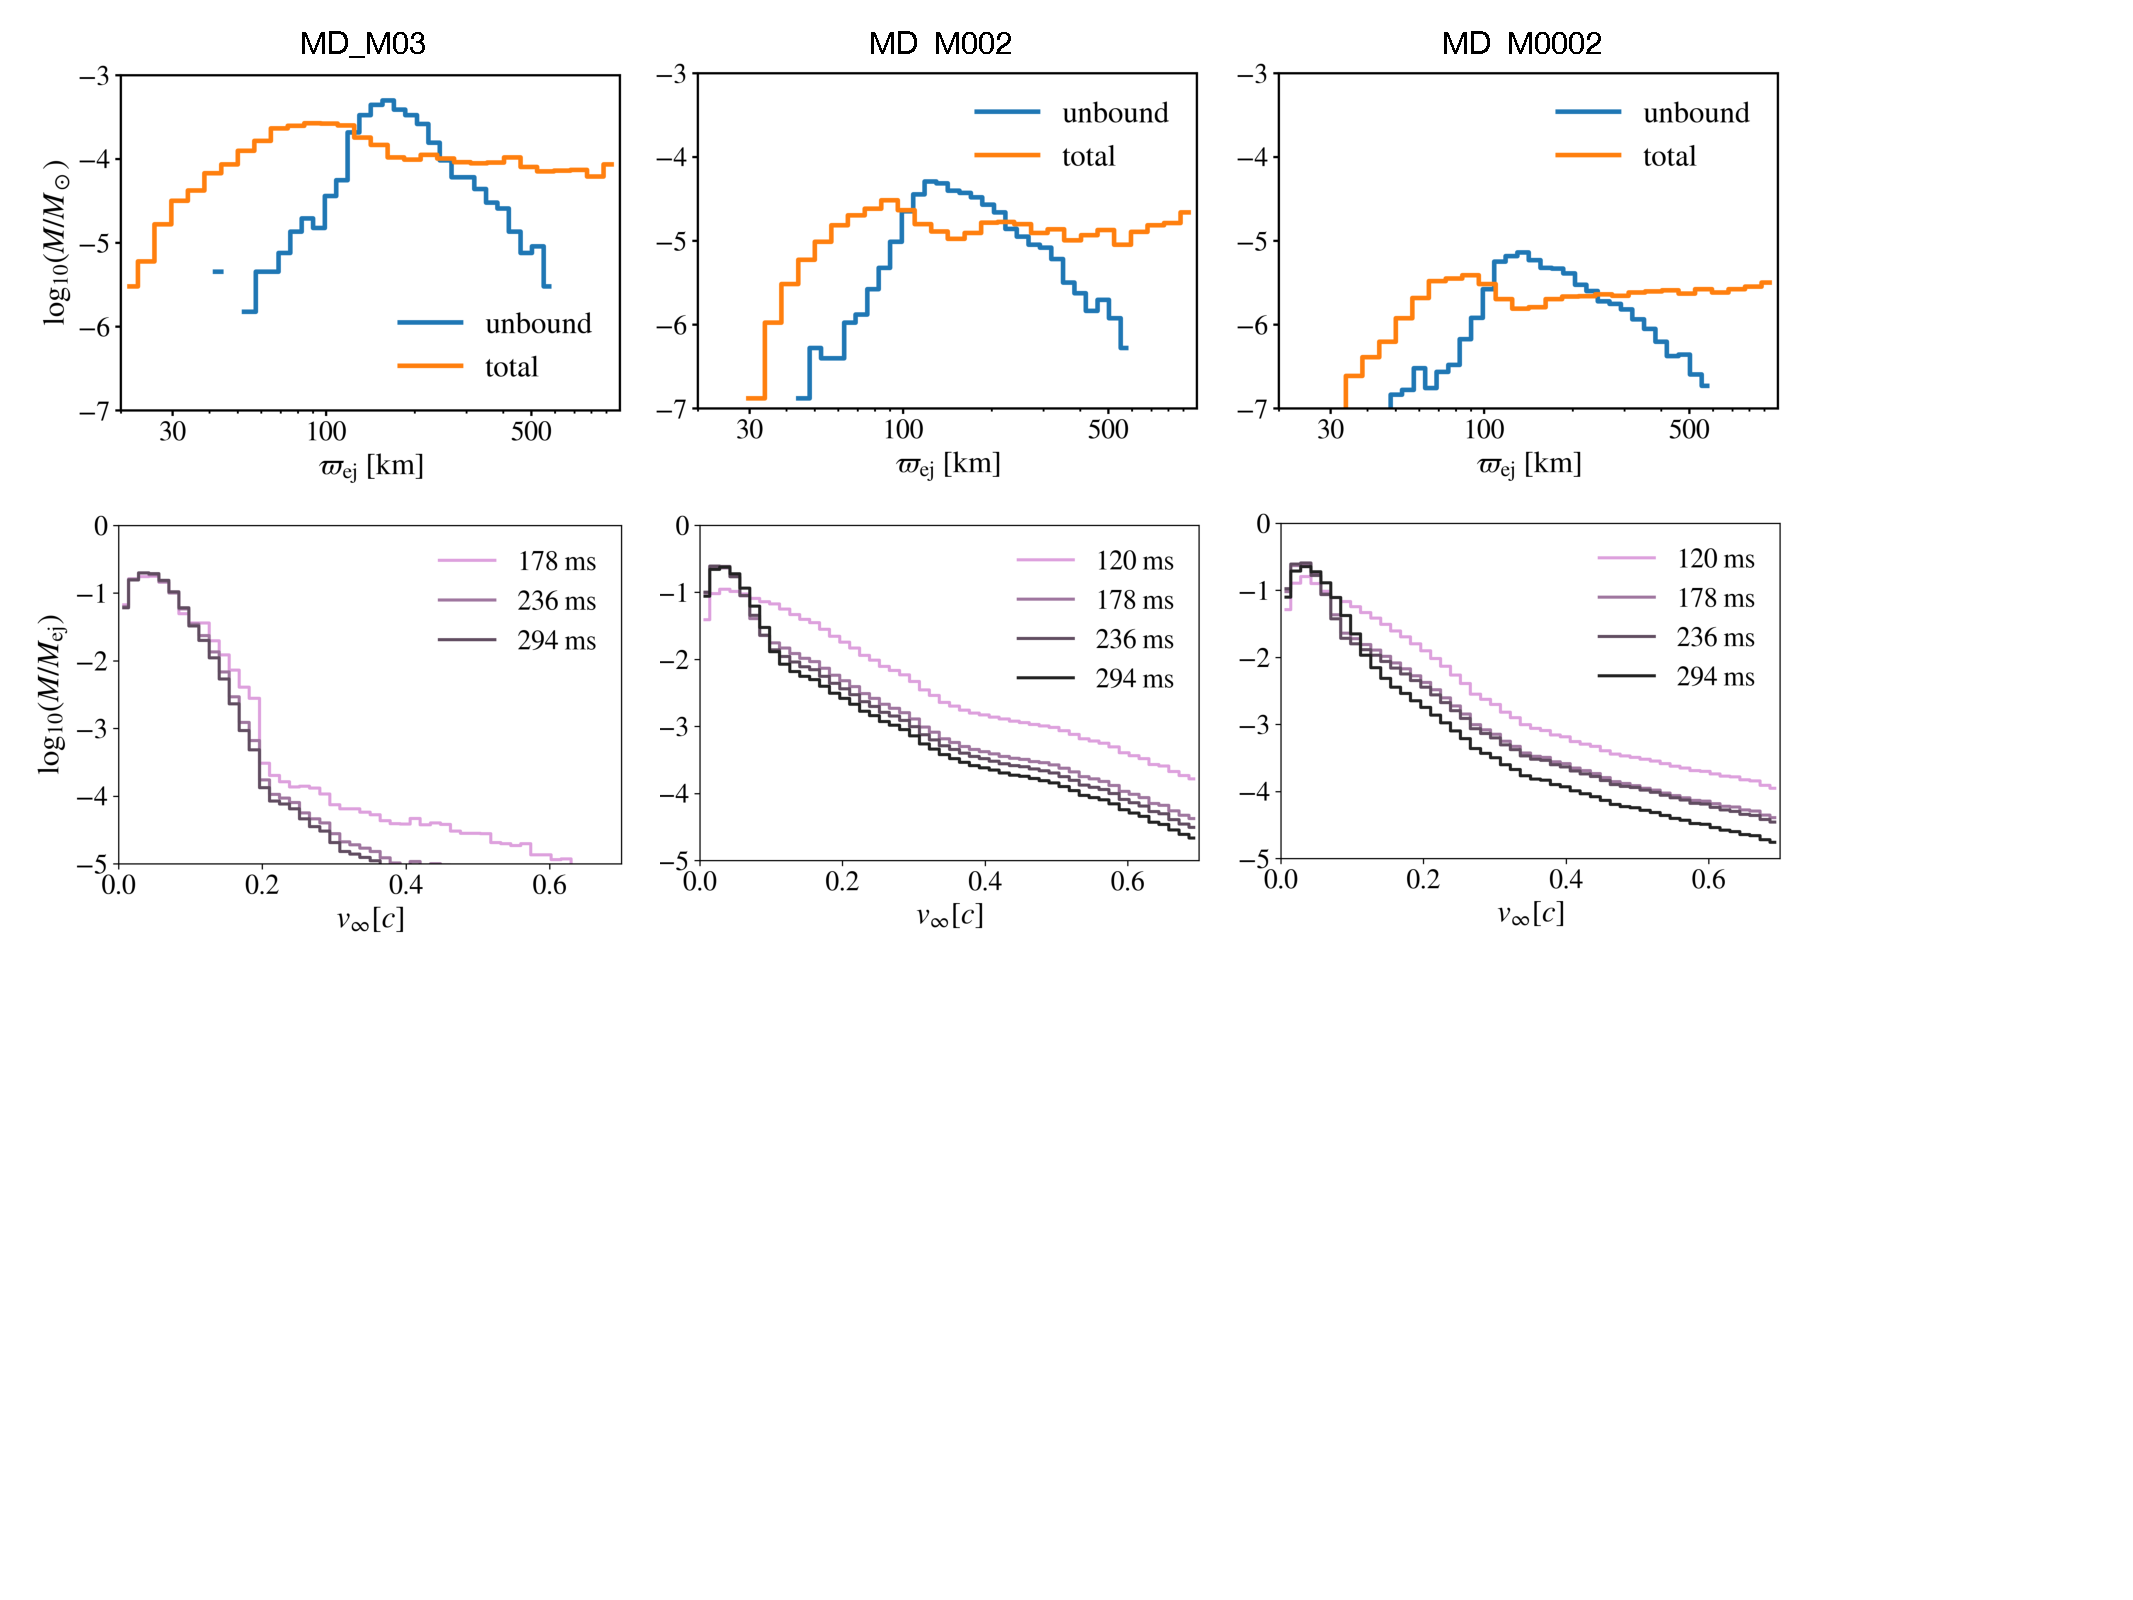
\includegraphics[width=\textwidth]{figures/kilonova/mass_vs_velocity_tracers_n_outflow.pdf}
 \caption{Outflow properties of the three accretion disks simulated in this work. Top: Mass distribution of unbound and total outflows as recorded by tracer particles in terms of their cylindrical radius $\varpi_{\rm ej}$ at which they get ejected from the disk corona. Bottom: Mass distributions of unbound outflows (normalized by the total disk outflow) in terms of their asymptotic escape velocities $v_\infty$. These measurements are performed by recording the properties of outflowing material through a spherical coordinate detector surface placed at a radius of 1034~km from the black hole.\label{fig:outflows}}
\end{figure*}

Outflows from the disks originate in high specific entropy (`hot') disk coronae as a result of an imbalance between heating and cooling at high latitudes. Viscous heating as well as dissipation of magnetic energy far from the midplane is not offset by neutrino cooling, which becomes energetically subdominant at the comparatively low densities off the midplane. The precise amount of material unbound from the disk depends on the details of the self-consistent heating-cooling imbalance generated by MHD turbulence. We refer to Ref. \cite{Siegel:2017jug} for a detailed discussion on the emergence of these outflows in the presence of MHD turbulence.

%Accretion of material onto the black hole causes an increase of density and temperature in the disk midplane. As neutrino emission follows density, these regions effectively participate in neutrino emission, which provide a cooling mechanism to balance the MHD heating. The rate of neutrino emission depends on the rate of accretion onto the black, as illustrated in Section \ref{sec:disk_composition}. Away from the disk midplane, the disk density drops rapidly, which causes a drop in the rate of neutrino emission. This creates an imbalance between the rate of heating from MHD turbulence and the rate of cooling from neutrino emission, resulting in regions of high entropy, which we refer to as the ``corona'', above and below the disk midplane. The low density corona regions then gives rise to strong outflows. 

We track properties of these outflows using $10^4$ tracer particles of equal mass, placed throughout the disk initially, with probability density proportional to the conserved rest mass density $\hat D = \sqrt \gamma \rho W$. The top panels of Fig.~\ref{fig:outflows} show the mass distribution of total and unbound disk outflow (ejecta) as recorded by the tracer particles in terms of the cylindrical radius at which the tracer particles are ejected from the disk corona, the latter begin defined as the cylindrical radius after which their radial coordinate position only increases with time. We define unbound material as having reached a coordinate radius of $10^3$\,km and additionally having positive specific energy at infinity, $-hu_t > 0$, where $h$ denotes the specific enthalpy and $u_0$ is the 0-component of the fluid four-velocity. For all simulations, we find that the total outflow material is almost evenly distributed over a broad  range of radii, whereas the majority of the ejecta mass originates from the inner accretion disk ($\varpi\lesssim100-250$~km), where most of the binding energy is released through viscous heating. The total amount of material ejected by the disks are $3.179\times 10^{-3}~M_\odot (\approx 10\%$ of the initial disk mass) for \texttt{MD\_M03}, $4.03\times 10^{-4}~M_\odot (\approx 20\%$ of the initial disk mass) for \texttt{MD\_M002}, and $6.046\times 10^{-5}~M_\odot (\approx 30\%$ of the initial disk mass) for \texttt{MD\_M0002} by the end of the simulations. The disks still generate steady winds at the end of our simulations, which indicates that the remaining disks would continue evaporating themselves if the simulations were evolved over longer timescales. Given that the total cumulative accreted masses have already converged over the duration of the simulation runs (cf.~Sec.~\ref{sec:accretion}), we predict that the remaining disk will generate outflow material corresponding to $\approx\! 37\%$ of the initial disk mass for \texttt{MD\_M03}, $\approx\! 18\%$ of the initial disk mass for \texttt{MD\_M002}, and $\approx\! 38\%$ of the initial disk mass for \texttt{MD\_M0002}. This material will be ejected over longer timescales by a combination of the MHD-driven outflows as discussed here and viscous spreading of the disk over several viscous timescales (see \cite{fernandez_long-term_2019} for a discussion of late-time viscous outflows).

The bottom panels of Figure \ref{fig:outflows} show the distribution of asymptotic ejecta velocity for the three simulation runs as measured from the mass flux through spherical coordinate detector surfaces placed at a radius of 1034\,km. The asymptotic velocities $v_\infty$ are computed from the asymptotic Lorentz factor $W_\infty = -hu_0$ as measured by the detector sphere. In all three simulations, we find the emergence of a high-velocity tail, with the bulk ejecta residing around $v_\infty\approx 0.1c$. This velocity scale is naturally explained as a combination of moderate outflow velocities from the hot corona of typically $(0.03-0.1)c$ together with the energy released by recombination of individual nucleons into $\alpha$-particles ($\approx\!7$\,MeV per baryon per $\alpha$-particle formed). Our velocity distributions are qualitatively similar to Refs. \cite{Fernandez:2018kax} and \cite{Christie:2019lim}, albeit their GRMHD run---similar to our \texttt{MD\_M03} case---shows more outflow mass at higher velocities; this has been commented on in Ref. \cite{Fernandez:2018kax} and can be attributed in part to their initial magnetic field configuration, which is optimized for fast magnetically-dominated outflows. The high-velocity tail for the low-$\dot{M}$ disks \texttt{MD\_M002} and \texttt{MD\_M0002} are more pronounced, which may be ascribed to more violent viscous heating as neutrino cooling becomes less important at low accretion rates.




\subsection{Weak interactions and disk composition}
\label{sec:disk_composition}

\begin{figure*}[t]
\centering
  \includegraphics[width=16cm]{figures/kilonova/snapshot_43_130_250_Ye_logetae_xy_MD_M03_M002_M0002.pdf}
 \caption{Snapshots of the electron fraction $Y_e$ and electron degeneracy $\eta=\mu_e/k_{\rm B}T$ over time for the three simulation runs performed here. Plotted are slices of these quantities in the disk midplane ($x$-$y$ plane) at times $t = 42.8$~ms, $t = 130$~ms, and $t = 250$~ms. Above the ignition threshold for weak interactions (Eq.~\eqref{eq:Mdot_ign_merger}), the high accretion rates of runs \texttt{MD\_M03} and \texttt{MD\_M002} cause the inner disk to remain strongly neutron-rich over time, whereas below the ignition threshold the low accretion rate of run \texttt{MD\_M0002} leads to accelerated protonization in the inner part. \label{fig:panels_Ye_eta}}
\vspace{5mm}
\end{figure*}


\begin{figure*}[t]
\centering
  \includegraphics[width=16cm]{figures/kilonova/snapshot_43_130_250_R_eff_nua_nue-entropy_xy_M03_M002_M0002.pdf}
 \caption{Evolution of the ratio of anti-electron to electron neutrino number emission rates $R_{\bar \nu_{\rm e}}^{\rm eff}/R_{\nu_{\rm e}}^{\rm eff}$ and specific entropy $s$ for the three simulation runs performed here. Plotted are snapshots of these quantities in the disk midplane ($x$-$y$ plane) at times $t = 42.8$~ms, $t = 130$~ms, and $t = 250$~ms.\label{fig:panels_R_eff_entropy}}
\vspace{5mm}
\end{figure*}

Accretion disks below and above the ignition threshold for weak interactions give rise to qualitatively different evolution of its composition as we shall illustrate in this section. Discussing weak interactions in the disk in more detail also benefits the interpretation of the behavior of some global disk quantities (Sec.~\ref{sec:global_properties}) as well as of nucleosynthesis in disk outflows (Sec.~\ref{sec:nucleosynthesis}).

Figures \ref{fig:panels_Ye_eta} and \ref{fig:panels_R_eff_entropy} show various quantities pertaining to the evolution of disk composition, including snapshots of the electron fraction, electron degeneracy $\eta=\mu_e/k_{\rm B}T$, where $\mu_e$ is the electron chemical potential, the ratio of $\bar{\nu}_e$ to $\nu_e$ number emission rates ($R_{\bar \nu_{\rm e}}^{\rm eff}/R_{\nu_{\rm e}}^{\rm eff}$), and specific entropy $s$ over the course of the three simulation runs.

Neglecting absorption of neutrinos, appropriate for the disk midplane, the weak interactions controlling disk composition are the charged-current $\beta$-processes,
\begin{eqnarray}\label{eq:proton_capture}
      e^- + p &\rightarrow& n + \nu_{\rm e}, \label{eq:proton_capture} \\
      e^+ + n &\rightarrow& p + \bar \nu_{\rm e}. \label{eq:neuton_capture}
\end{eqnarray}
Starting off from neutron-rich initial conditions $Y_e\approx 0.1$ (cf.~Sec.~\ref{sec:methods}), one expects the disks to protonize over time due to Eq.~\eqref{eq:neuton_capture} dominating. This is evident from $R_{\bar \nu_{\rm e}}^{\rm eff}/R_{\nu_{\rm e}}^{\rm eff}>0$ and the gradual increase of $Y_e$ over time of in the outer parts of the accretion disks in Figs.~\ref{fig:panels_R_eff_entropy} and \ref{fig:panels_Ye_eta}. However, less massive disks with lower $\dot{M}$ such as \texttt{MD\_M002} and \texttt{MD\_M0002} take longer times compared to \texttt{MD\_M03} to raise their electron fraction from its initial value; this can be understood from an analysis of the disk protonization timescale.

From the equations of lepton number and baryon number conservation, we
compute
\begin{equation}
  R = \nabla_\mu(n_e u^\mu) = \nabla_\mu(n_{\rm b} u^\mu Y_e) = n_{\rm b} u^\mu
  \nabla_\mu Y_e,
\end{equation}
and thus
\begin{equation}
  u^\mu \nabla_\mu Y_e = R \frac{m_{\rm b}}{\rho}, \label{eq:Y_e_cons}
\end{equation}
where $u^\mu$ is the four-velocity of the fluid and $R$ denotes a source term to account for the change in lepton number due to weak interactions. Equation \eqref{eq:Y_e_cons} shows that along a fluid trajectory, i.e., in the comoving frame of the fluid, the electron fraction changes by a rate of $R m_{\rm b}/ \rho$. We can therefore define the characteristic timescale for the composition of matter to change by $t_{Y_e} \equiv Y_e\rho / (R m_\mathrm{b})$. Neglecting neutrino absorption, appropriate for the disk midplane, one has
\begin{equation}
  t_{Y_e} = \frac{Y_e}{R_{\bar{\nu_e}}^\mathrm{eff} -
    R_{\nu_e}^\mathrm{eff}}\frac{\rho}{m_{\rm b}}. \label{eq:t_Ye}
\end{equation}
Ignoring final state blocking in the neutrino phase space, the effective emission rates scale as \cite{tubbs_neutrino_1975,bruenn_stellar_1985} $R_{\bar{\nu}_e,\nu_e}^\mathrm{eff} \propto \rho T^5 \propto \dot{M}^{9/4}$, where we have used the approximate expression Eq.~\eqref{eq:T_1D} for the midplane temperature in the second step. Furthermore, since $\dot{M}\propto \rho$ (cf.~Eq.~\eqref{eq:Mdot_1D_2}), we deduce that, approximately,
\begin{equation}
  t_{Y_e} \propto \dot{M}^{-5/4},  \label{eq:t_Ye_scale_Mdot}
\end{equation}
which explains the decrease in protonization timescale with increasing accretion rate seen in the outer accretion disks in Figs.~\ref{fig:panels_Ye_eta} and \ref{fig:panels_R_eff_entropy}.

The inner accretion disk shows qualitatively different behavior depending on whether the accretion disk resides in a state above or below the ignition threshold (Eq.~\eqref{eq:Mdot_ign_merger}, Sec.~\ref{sec:neutrino_emission}). We find that above the ignition threshold, the disk midplane density $\rho\propto \dot{M}$ (cf.~Eq.~\eqref{eq:Mdot_1D_2}) is sufficiently large that electrons become degenerate, as shown in Fig.~\ref{fig:panels_Ye_eta}. This, in turn, suppresses positron creation via $\gamma\rightarrow e^+ + e^-$ and thus Eq.~\eqref{eq:neuton_capture} relative to \eqref{eq:proton_capture}, and hence leads to slight neutronization even in very neutron-rich initial conditions (see \texttt{MD\_M03} in Fig.~\ref{fig:panels_R_eff_entropy}). This neutronization mechanism is also the reason why collapsar accretion disks starting with much higher $Y_e$ were found to be able to generate neutron-rich outflows and synthesize r-process elements \cite{siegel_collapsars_2019}. However, the inner parts of the accretion disks cannot become arbitrarily degenerate and neutron rich, thanks to a self-regulation mechanism discussed in Ref. \cite{Siegel:2017jug} and previously pointed out by Ref. \cite{chen_neutrino-cooled_2007}. As shown in Fig.~\ref{fig:panels_Ye_eta}, disk self-regulation leads to a heating-cooling balance that results in moderate electron degeneracy $\eta\sim 1$ and corresponding neutron richness of $Y_e\approx 1$. At lower $\dot{M}$, close to the ignition threshold, degeneracy and self-regulation become somewhat weaker and less pronounced; however, \texttt{MD\_M002} still qualitatively shows the same behavior as \texttt{MD\_M03}. We also note that as a result of viscous spreading, the disk density decreases over time, which may suppress degeneracy eventually late in the disk's evolution. The onset of a decrease in degeneracy is noticeable from the snapshots in Fig.~\ref{fig:panels_Ye_eta}. However, by the time massive disks such as \texttt{MD\_M03} reach this break-down of degeneracy, most disk material has been evaporated and the change in disk composition has little effect on the overall composition of ejecta. While the disk is in such a self-regulated, moderately degenerate phase, the inner part of the accretion disk feeds highly neutron-rich material into the outflows.

Below the ignition threshold, we find an inverted scenario in terms of midplane composition within the inner parts of the accretion disk. The timescale for protonization in the innermost part of the accretion disk is significantly smaller than in the outer parts, resulting in a high-$Y_e$ surrounding of the black hole already at $t\sim100$\,ms (cf.~\texttt{MD\_M0002} in Fig.~\ref{fig:panels_Ye_eta}). We attribute this to excess viscous heating in the absence of energetically significant neutrino cooling. The resulting high-entropy environment (cf.~Fig.~\ref{fig:panels_R_eff_entropy}) leads to a prolific generation of positrons via pair production, $\gamma\rightarrow e^+ + e^-$, and thus decreases the timescale for protonization via Eq.~\eqref{eq:neuton_capture}. This innermost region in \texttt{MD\_M0002} is too small, however, to feed material into the outflows sufficient enough for a pronounced high-$Y_e$ tail of the ejecta (cf.~Sec.~\ref{sec:nucleosynthesis}).


%Figure \ref{fig:panels_Ye_eta} shows the variation of the electron fraction $Y_e$ and the electron degeneracy $\eta$, and \ref{fig:panels_R_eff_entropy} shows the variation of the ratio of neutrino number emission rate to antineutrino number emission rate and entropy over the course of the threes simulations. We find that the overall pattern of variation of disk properties in terms of these parameters are similar for the high disk mass cases \texttt{MD\_M03} and \texttt{MD\_M002}, where weak interactions are important. For the lowest disk mass case \texttt{MD\_M0002}, we see a difference in the disk properties, determined by negligible weak interactions. We notice that for \texttt{MD\_M03} and \texttt{MD\_M002}, the disks have low $Y_{\rm e}$ inside and high $Y_{\rm e}$ outside, whereas for \texttt{MD\_M0002}, the pattern reverses, with the inner disk having high $Y_{\rm e}$ and the outer disk having low $Y_{\rm e}$. The disk physics is controlled by the following processes:
%\begin{enumerate}[i)]
%  \item charged current $\beta$-processes \\
%  \begin{equation}\label{eq:proton_capture}
%      e^- + p \rightarrow n + \nu_{\rm e}
%  \end{equation}
%  \begin{equation}\label{eq:neuton_capture}
%      e^+ + n \rightarrow p + \bar \nu_{\rm e}
%  \end{equation}
%  \item electron-positron pair production
%  \begin{equation}\label{eq:pair_prod}
%      \gamma \rightarrow e^+ + e^-
%  \end{equation}
%\end{enumerate}

%In \texttt{MD\_M03} and \texttt{MD\_M002}, Equation \ref{eq:neuton_capture} is favored in the outer disks, as the disks start neutron rich, causing this region to protonize over time, increasing the ratio of $\bar \nu_{\rm e}$ to $\nu_{\rm e}$ production. The decreasing $\nu_{\rm e}$ production decreases the amount of cooling, causing the entropy to rise over time. $\dot M$ in these simulations is fairly high, leading to high densities in the inner disks. The high density causes $e^-$ degeneracy, and inhibits Equation \ref{eq:pair_prod}. The lack of $e^+$ production suppresses Equation \ref{eq:neuton_capture}, and the disk neutronizes over time.

%For \texttt{MD\_M0002}, $\dot M$ is significantly low, leading to very low density in the inner disk. As $\nu_{\rm e}$ emission tracks density, this leads to the absence of $\nu_{\rm e}$ cooling, and as a result, an increase in entropy. The high entropy causes Equation \ref{eq:pair_prod} to proceed efficiently. The increased amount of $e^+$ produced stimulates Equation \ref{eq:neuton_capture}, protonizing the disk over time. In the outer disk, \ref{eq:neuton_capture} is again is expected to be favored over \ref{eq:proton_capture}, as the disk starts neutron rich. However, there is no pile up of heat in this region, due to which the rates of these reactions are low.

%Although \ref{eq:neuton_capture} is favored over \ref{eq:proton_capture} throughout the simulation, in the inner disk, the sufficient amount of 






\subsection{Nucleosynthesis}
\label{sec:nucleosynthesis}

\begin{figure}[t]
  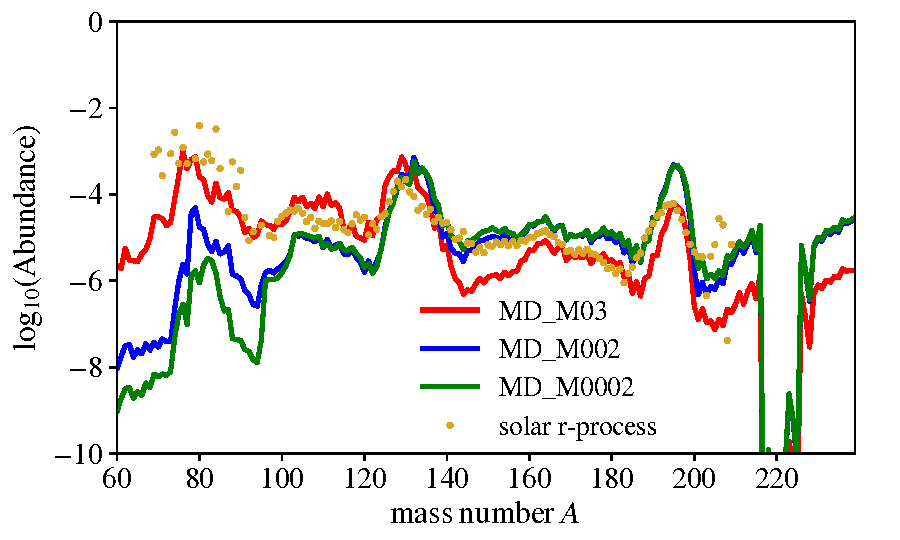
\includegraphics[width=\columnwidth]{figures/kilonova/final_abundances_sims_comparison_MD_M03-MD_M002-MD_M0002.pdf}
 \caption{Final elemental abundances at $10^9$\,s for the accretion disk ejecta of our three simulation runs. Shown are mean abundances of all unbound tracer particles (excluding the disk relaxation phase). Also plotted for reference are the observed solar system abundances from Ref. \cite{arnould_$r$-process_2007}, scaled to match the \texttt{MD\_M03} abundance at $A = 195$. \label{fig:abundances}}
\end{figure}

\begin{figure}[t]
  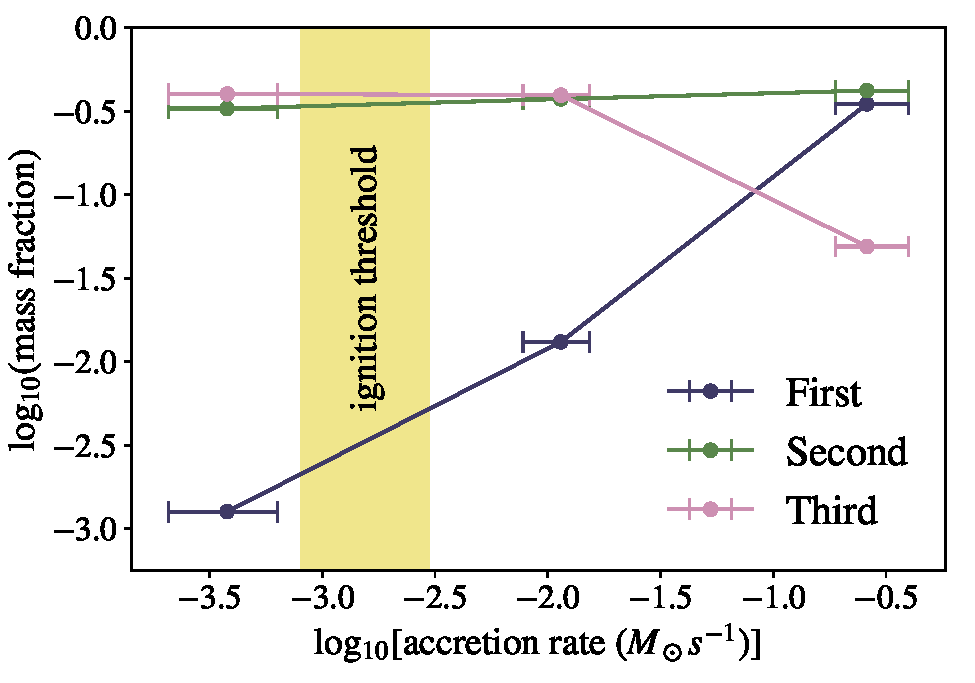
\includegraphics[width=\columnwidth]{figures/kilonova/mass_fraction_peaks.pdf}
 \caption{Mass fractions of the nucleosynthetic yields in
the first (summed over $A=70-90$), second (summed over $A=125-135$), and third (summed over $A=186-203$) r-process peaks for the disk ejecta of simulation runs \texttt{MD\_M03}, \texttt{MD\_M002}, and \texttt{MD\_M0002} presented here. A qualitative change in nucleosynthesis products across the ignition threshold for weak interactions (Eq.~\eqref{eq:Mdot_ign_merger}) is evident. \label{fig:mass_frac_peaks}}
\end{figure}

\begin{figure}[t]
  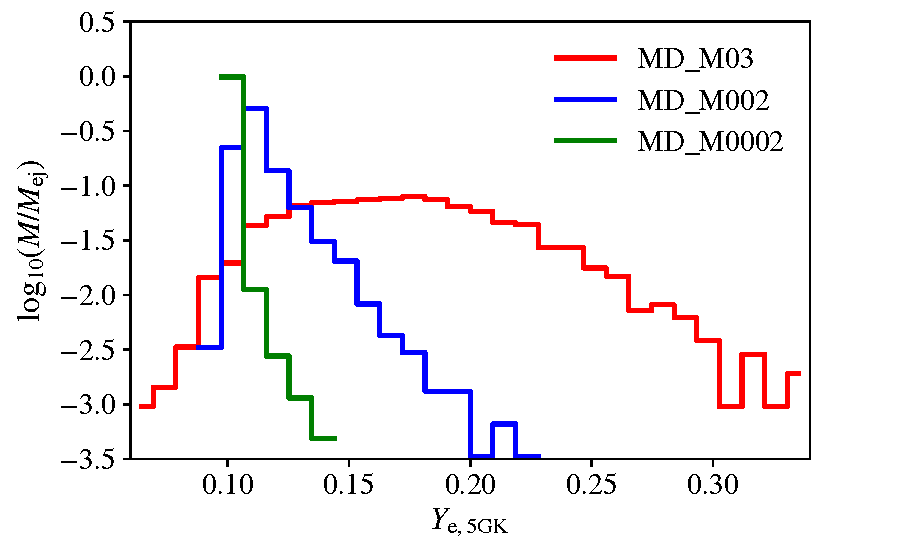
\includegraphics[width=\columnwidth]{figures/kilonova/Ye_sims_comparison_MD_M03-MD_M002-MD_M0002.pdf}
 \caption{Mass distribution of unbound outflows from our simulated accretion disks according to the electron fraction $Y_{\rm e}$, extracted from tracer particles at 5\,GK. A significant high-$Y_e$ tail is established across the ignition threshold. \label{fig:mass-Ye-outflow}}
\end{figure}

The neutron-rich outflows generated by our post-merger accretion disks are sites for r-process nucleosynthesis. We record thermodynamic properties of the ejecta by tracer particles distributed throughout the disks initially (cf.~Sec.~\ref{sec:ejecta}), and use such tracer profiles as input to nuclear reaction network calculations. The initial conditions important to the outcome of the r-process are set mostly by the electron fraction, specific entropy, and expansion timescale of the flow at $T\approx 5$\,GK \cite{lippuner_r-process_2015}, which is the characteristic temperature at which nuclear statistical equilibrium breaks down, and neutron-capture reactions set in.

Neutrino absorption is taken into account approximately by a ring-like `light-bulb' scheme in post-processing \cite{fernandez_delayed_2013}, which irradiates the ejecta with neutrino luminosities as computed in Sec.~\ref{sec:neutrino_emission}. We refer to Ref. \cite{fernandez_delayed_2013} and Ref. \cite{Siegel:2017jug} for more details on this approach.

Starting at 10~GK, we perform full nuclear reaction network calculations on the tracer particles using the reaction network \texttt{SkyNet}~\cite{lippuner_skynet:_2017}, in order to track nuclear abundances as the outflows undergo r-process nucleosynthesis. Figure \ref{fig:abundances} shows the final total abundance yields from all tracers after $10^9$\,s for all three disk simulation runs. These abundances are the result of integrated ejecta that are unbound over the course of the simulation runs, most of which originate from the inner accretion disk region with radii between $\approx(100-250)$~km (cf.~Fig.~\ref{fig:outflows}). 

Final r-process abundance patterns qualitatively change across the ignition threshold for weak interactions in post-merger disks (see Fig.~\ref{fig:abundances}). At high accretion rates, such as run \texttt{MD\_M03}, we find abundances in good agreement with residual solar r-process abundances~\cite{arnould_$r$-process_2007} across the entire range of mass numbers from the first ($A\approx80$) to the third ($A\approx195$) r-process peak (see \cite{Siegel:2017jug} for a more detailed discussion on this case). While across all accretion rates we find good agreement with the solar abundance pattern between the second peak ($A\approx130$) and the third r-process peak, run \texttt{MD\_M002} (close to the ignition threshold) already shows somewhat suppressed first-to-second peak elements, and light r-process elements are strongly suppressed below the ignition threshold (run \texttt{MD\_M0002}).

The qualitative change in nucleosynthesis patterns across the ignition threshold is further illustrated by Fig.~\ref{fig:mass_frac_peaks}, which shows the mass fractions of nuclei grouped into first-, second- and third-peak elements as a function of accretion rate. While 2nd-peak elements are synthesized in roughly constant amounts across the $\dot{M}$ range investigated here, abundances of light r-process nuclei rise strongly toward and around the ignition threshold, while 3rd-peak nuclei are somewhat overproduced in that regime.

This behavior is a result of a qualitative change in the distribution of $Y_e$ of the ejecta across the ignition threshold as evident from Fig.~\ref{fig:mass-Ye-outflow}. While at low $\dot{M}$, below the ignition threshold, the $Y_e$ distribution of the unbound outflows at 5\,GK is still centered around the initial value of $Y_e=0.1$ (run \texttt{MD\_M0002}), run \texttt{MD\_M002} close to the ignition threshold has already built up a significant tail toward higher electron fraction; finally, run \texttt{MD\_M03} shows a broad distribution of $Y_e$ at least up to $\lesssim 0.4$. This effect can be  ascribed in part to the strongly changing protonization timescale as a function of accretion rate across the ignition threshold (cf.~Eq.~\eqref{eq:t_Ye_scale_Mdot}; Sec.~\ref{sec:disk_composition}). There is a possibility of our tracer particles slightly under-resolving the high-$Y_e$ tail---a significantly larger number of tracers, excluded here due to computational cost and feasibility, may better resolve the effects of, e.g., an inner high-$Y_e$ part of the \texttt{MD\_M0002} disk, but is unlikely to qualitatively change the  conclusion reached here. Toward high $\dot{M}$, neutrino absorption by the ejecta contributes to flattening the $Y_e$ distribution as well. This effect is already noticeable for \texttt{MD\_M03} and is expected to become more important at even higher $\dot{M}$ disks \cite{miller_full_2019-1}, which are beyond the scope of the present paper.



%The nucleosynthetic yields of the three models can be understood with the help of Figure \ref{fig:panels_Ye_eta} and Figure \ref{fig:mass-Ye-outflow}. Figure \ref{fig:mass-Ye-outflow} shows the mass distribution of unbound outflows measured by tracer particles in terms of $Y_{\rm e}$. Ejecta from all three models can be seen to be comprised of significant amounts low $Y_{\rm e}$ material, $\approx(0.1-0.15)$, due to the initial disks being set to $Y_{\rm e} = 0.1$. % for a significant part in the outflows over time.
%For \texttt{MD\_M03} and \texttt{MD\_M002} this low $Y_{\rm e}$ material is generated from the inner disks, and for \texttt{MD\_M0002} from the outer disk, as observed in Figure \ref{fig:panels_Ye_eta}. As low $Y_{\rm e}$ corresponds to large number of free neutrons, this outflow material enables the $r$-process to generously produce high mass number nuclei. As the disk mass is increased, the ejecta can be seen to be spanning over of a broader range of $Y_{\rm e}$ material, such that the average values of $Y_{\rm e}$ is 0.101~erg s$^-1$ for \texttt{MD\_M0002}, 0.114~erg s$^-1$ for \texttt{MD\_M002}, and 0.174~erg s$^-1$ for \texttt{MD\_M03}.

%For \texttt{MD\_M03}, there is significant amount of neutrino production in the disk midplane. These neutrinos further change the composition of a part of the outer disks and the outflows, resulting in the addition sufficient high $Y_{\rm e}$ material--- corresponding to low mass nuclei---as well in the outflows. High $Y_{\rm e}$ implies availability of few amounts of free neutrons, disabling the $r$-process from producing high mass nuclei.

%For \texttt{MD\_M002}, the reduced amount of neutrino emission in the disk midplane, due to a lower accretion rate compared to \texttt{MD\_M03}, does not sufficiently change the composition of the outflows. The reduced conversion of low $Y_{\rm e}$ material to high $Y_{\rm e}$ material reduces the amount of production of low mass nuclei.

%For \texttt{MD\_M0002}, although the inner disk produces high $Y_{\rm e}$ material, they are not produced in significant amounts. The weak interactions in the inner disk in this model is not efficient enough to contribute strongly to the production of low mass nuclei. Additionally, neutrino emission being nearly absent in the disk midplane leads to a negligible conversion of low $Y_{\rm e}$ material produced by the outer disk to high $Y_{\rm e}$ material. These reasons combined explains the significant drop in the production of low mass nuclei, by about an order of magnitude lower as compared to \texttt{MD\_M002}.   


%Lots of n rich material, lots of lanthanides in lowest $\dot M$. How much ejecta do we get in the three cases?

%How much elements in each peak?

%Do we get/not get blue kilonova?

%Nucleosynthesis trends in second and third peaks.

%Do we get blue ejecta at all in MD\_M0002? Here, it'll come from the inner part.

%As we cross ignition threshold, we see where blue/red component is coming from.

%Blue ejecta component from outside, red component from inside.


%\section{Section 4}
%High velocity tail discussion. Which plots here?

%\section{Section 5}
%Summarize results in terms of future mergers.

\section{Conclusion}
\label{sec:conclusion}

%Discussion in the light of GW190425: low-mass accretion disks expected! Discuss disk outflow/mass in comparison with other ejecta channels for such high-mass NS-NS systems. Can we predict any kilonova estimates (would need kilonova model, will require extra work)?

Our simulation results provide important implications for the electromagnetic counterpart observables of LIGO-Virgo's source population BNS and NSBH mergers. As presented in Section \ref{sec:nucleosynthesis}, all three of our models produce heavy $r$-process elements---corresponding to red kilonova components, with our highest disk model being able to produce light $r$-process elements as well. Our results indicate that nucleosynthetic yields from postmerger accretion disks comprising primarily of light $r$-process elements, corresponding to a strong blue kilonova would require fairly high disk masses, such as the model in Ref. \cite{miller_full_2019-1}. As shown in Section \ref{sec:param_space}, high disk masses would result from small total masses for binary systems. The observation of a blue kilonova would be possible from very low mass BNS systems, and is unlikely from NSBH systems. The second LIGO-Virgo BNS detection, GW190425, was not accompanied by any electromagnetic counterparts. However, with binary total mass being one of the parameters that is accurately measured by gravitational-wave observations, this binary has been concluded to belong to the high mass regime of the neutron star binary parameter space. In such a scenario, our simulation results predict production of heavy $r$-process elements in the nucleosynthetic yields of the remnant accretion disks, resulting in a red kilonova. The system being located at significantly larger distances compared to the first BNS candidate, GW170817, in addition to the poor sky localization of the event, would account for the inability in detecting the kilonova signatures. 

\section{Appendix}
\subsection{Ignition threshold}
\label{app:ignition_threshold}

The basic scaling $\dot{M}_{\rm ign}\propto \alpha_{\rm visc}^{5/3}$ (cf.~Eq.~\eqref{eq:Mdot_ign}) of the accretion rate at the ignition threshold for weak interactions in an accretion disk with the dimensionless, effective Shakura-Sunyaev viscosity coefficient $\alpha_{\rm visc}$ can be derived analytically. To this end, we work within a height-integrated, one-dimensional model for accretion disks in Kerr spacetime with metric $g_{\mu\nu}$ using Boyer-Lindquist coordinates $x^i = (t,r,\theta, \phi)$ (e.g., \cite{beloborodov_super-eddington_1998,gammie_advection-dominated_1998,chen_neutrino-cooled_2007}). In such 1D models, angular averages are performed by approximating $\int {\rm d}\theta {\rm d}\phi \sqrt{g} q \simeq 4\pi H q(\theta = \pi/2)$, where $q$ represents any physical quantity, $H(r)$ is the characteristic angular half-thickness of the disk, and $g = {\rm det}(g_{\mu\nu})$. We work in the ``thin-disk'' approximation \cite{shakura_black_1973,bardeen_rotating_1972,novikov_astrophysics_1973}, well justified if neutrino cooling is significant, in which terms in $(H/r)^2$ are neglected and gas pressure is negligible, resulting in the assumption that the fluid orbits with four-velocity $u^\mu = (u^t,u^r, 0, u^\phi)$ and Keplerian angular velocity $\Omega \equiv u^\phi/u^t = c/(r\sqrt{2r/r_{\rm g}} + \chi_{\rm BH} r_{\rm g}/2)$. Here, $r_{\rm g}=2GM/c^2$ is the gravitational radius, and $M_{\rm BH}$ and $\chi_{\rm BH}$ denote, as before, the mass and the dimensionless spin of the black hole, respectively. In this thin-disk limit, the equation of vertical hydrodynamical equilibrium for the disk, can be written as (cf.~\cite{abramowicz_accretion_1997,beloborodov_super-eddington_1998})

\begin{equation}
	\left(\frac{H}{r}\right)^2 = \frac{2 r}{c^2 r_{\rm g} J(\chi_{\rm BH},r)}\frac{p}{\rho},\mskip40mu \text{or} \mskip40mu c_{\rm s} = c\left(\frac{J(\chi_{\rm BH},r) r_{\rm g}}{2r}\right)^{\frac{1}{2}}\frac{H}{r}, \label{eq:vertical_equilibrium}
\end{equation}

where $c_{\rm s}=\sqrt{p/\rho}$ is the isothermal sound speed, and
\begin{equation}
	J(\chi_{\rm BH},r) \equiv \frac{2\left(r^2 - \chi_{\rm BH} r_{\rm g}\sqrt{2r_{\rm g}r}+ 3\chi_{\rm BH}^2 r_{\rm g}^2 / 4 \right)}{2r^2 - 3r_{\rm g}r + \chi_{\rm BH} r_{\rm g}\sqrt{2r_{\rm g}r}}.
\end{equation}
The equation of baryon number conservation reads
\begin{equation}
	\dot{M} = -2\pi r c u^r \Sigma, \label{eq:baryon_conservation}
\end{equation}
where $\Sigma = 2H\rho$ is the disk surface density. From the equations of energy and angular momentum conservation, one can derive the identity \cite{page_disk-accretion_1974,chen_neutrino-cooled_2007}
\begin{equation}
	2\nu \Sigma r \sigma^{r}_\phi = -\frac{c r_{\rm g}}{4\pi} \dot{M} F(x,\chi_{\rm BH}), \label{eq:shear_identity}
\end{equation}
where $\nu$ is the kinematic viscosity, $\sigma^r_\phi = (1/2) c g^{rr} g_{\phi\phi}\sqrt{-g^{tt}}\gamma^3 ({\rm d}\Omega/{\rm d}r)$ is the shear, with $\gamma=u^t/\sqrt{-g^{tt}}$ being the Lorentz factor of the fluid measured by a zero-angular momentum observer, and
%\begin{eqnarray}

\begin{equation}
\begin{split}
F(x,\chi_{\rm BH}) \equiv \frac{x^3 + \chi_{\rm BH}}{(x^3 - 3x + 2\chi_{\rm BH})^{1/2}x^{3/2}} \Bigg[ (x-x_0)-\frac{3}{2}\chi_{\rm BH} \ln\frac{x}{x_0}- \\ \frac{3(x_1-\chi_{\rm BH})^2}{x_1(x_1-x_2)(x_1-x_3)}\ln\left(\frac{x-x_1}{x_0-x_1}\right) - \frac{3(x_2-\chi_{\rm BH})^2}{x_2(x_2-x_1)(x_2-x_3)}\ln\left(\frac{x-x_2}{x_0-x_2}\right) - \\ \frac{3(x_3-\chi_{\rm BH})^2}{x_3(x_3-x_1)(x_3-x_2)}\ln\left(\frac{x-x_3}{x_0-x_3}\right)\Bigg]. \label{eq:F_x}
\end{split}
\end{equation}
%\end{eqnarray}

Here, $x\equiv \sqrt{2r/r_{\rm g}}$, $x_0$ corresponds to the location of the marginally stable orbit, and $x_1$, $x_2$, $x_3$ are the roots of $x^3-3x+2\chi_{\rm BH}=0$. Explicitly, $x_1=2\cos(\frac{1}{3}\cos^{-1}\chi_{\rm BH}-\pi/3)$, $x_2=2\cos(\frac{1}{3}\cos^{-1}\chi_{\rm BH}+\pi/3)$, and $x_3=-2\cos(\frac{1}{3}\cos^{-1}\chi_{\rm BH})$.
Substituting Eq.~\eqref{eq:shear_identity} into Eq.~\eqref{eq:baryon_conservation} and using Eq.~\eqref{eq:vertical_equilibrium} one finds
\begin{equation}
	u^r = \frac{8}{3} \left(\frac{J(r,\chi_{\rm BH}) r}{2c^2 r_{\rm g}}\right)^{\frac{1}{2}} \frac{\sigma^r_\phi}{F(x,\chi_{\rm BH})}\alpha \left(\frac{H}{r}\right)^2, 
\end{equation}
where we have adopted the Shakura-Sunyaev parametrization $\nu = \frac{2}{3}\alpha_{\rm visc} c_{\rm s} H$ with viscosity coefficient $\alpha_{\rm visc}$. Substituting this back into Eq.~\eqref{eq:baryon_conservation}, we obtain
\begin{eqnarray}
	\dot{M} &=& - \frac{32\pi r_{\rm g}^2}{3\sqrt{2}} J^{\frac{1}{2}}(r,\chi_{\rm BH}) \left(\frac{r}{r_{\rm g}}\right)^{\frac{5}{2}} \frac{\sigma^r_\phi}{F(x,\chi_{\rm BH})}\alpha \rho \left(\frac{H}{r}\right)^3  \label{eq:Mdot_1D_1} \\
		&=& 2\sqrt{2}\pi c r_{\rm g}^2 S^{-1}(r,\chi_{\rm BH}) J^{\frac{1}{2}}(r,\chi_{\rm BH})  \left(\frac{r}{r_{\rm g}}\right)^{\frac{3}{2}} \alpha \rho \left(\frac{H}{r}\right)^3,  \label{eq:Mdot_1D_2}
\end{eqnarray}
where we have introduced the function $S(r,\chi_{\rm BH})=-(3/8)c(r_{\rm g}/r) [F(x,
\chi_{\rm BH})/\sigma^r_\phi]$, which varies between zero at the marginally stable orbit $x_0$ and unity at $r\rightarrow\infty$.

Viscous heating rate per unit area of the disk is given by $Q^+ = 2\nu\Sigma h c \sigma^r_\phi \sqrt{-g^{tt}}\gamma ({\rm d}\Omega/{\rm d}r)$, where $h\approx 1$ is the specific enthalpy of the fluid in the thin disk \cite{beloborodov_super-eddington_1998}. Using the identity \eqref{eq:shear_identity} one can rewrite this as
\begin{equation}
	Q^+ = \frac{c^2}{4\pi}\left(\frac{r}{r_{\rm g}}\right)^{-1} F(x,\chi_{\rm BH}) \mathcal{Q}(r,M_{\rm BH},\chi_{\rm BH}) \dot{M}, \label{eq:Qplus}
\end{equation}
where $\mathcal{Q}(r,M_{\rm BH},\chi_{\rm BH})\equiv -u^t ({\rm d}\Omega/{\rm d}r)$. We assume that cooling of the disk is dominated by electron and positron capture (URCA cooling). Ignoring final state blocking in the neutrino phase space, the cooling rate per unit area of the disk is then approximately given by \cite{tubbs_neutrino_1975,bruenn_stellar_1985,qian_nucleosynthesis_1996,popham_hyperaccreting_1999}
\begin{equation}
	Q^-_\nu = 2H \mathcal{C}_\nu \rho T^6. \label{eq:Qminus_nu_def}
\end{equation}
Here, $\mathcal{C}_\nu$ is a constant times the mass fraction of nucleons $X_{\rm nuc}$, which is roughly unity in the inner parts of the accretion disk where photodisintegration breaks down nuclei into neutrons and protons once $T\sim 10^{10}$\,K. At sufficiently small $\dot{M}$ (low midplane density), the pressure is dominated by radiation pressure, $p = \frac{11}{12}a_{\rm SB} T^4$, where contributions of relativistic electron-positron pairs have been included \cite{popham_hyperaccreting_1999}. Substituting into Eq.~\eqref{eq:vertical_equilibrium}, this yields the disk midplane temperature
\begin{equation}
	T = \left(\frac{6}{11}\frac{c^2}{a_{\rm SB}}\right)^{\frac{1}{4}} J^{\frac{1}{4}}(r,\chi_{\rm BH}) \left(\frac{r}{r_{\rm g}}\right)^{-\frac{1}{4}} \left(\frac{H}{r}\right)^{\frac{1}{2}} \rho^{\frac{1}{4}}. \label{eq:T_1D}
\end{equation}
Using this relation in Eq.~\eqref{eq:Qminus_nu_def} together with Eq.~\eqref{eq:Mdot_1D_2}, one obtains the following expression for neutrino cooling:
\begin{equation}
	Q^-_\nu = 2 \mathcal{C}_\nu \left(\frac{1}{2\sqrt{2}\pi c}\right)^{\frac{5}{2}} \left(\frac{6}{11}\frac{c^2}{a_{\rm SB}}\right)^{\frac{3}{2}} r_{\rm g}^{-4} S^{\frac{5}{2}}(r,\chi_{\rm BH}) J^{\frac{1}{4}}(r,\chi_{\rm BH}) \left(\frac{r}{r_{\rm g}}\right)^{-\frac{17}{4}}\left(\frac{H}{r}\right)^{-\frac{7}{2}} \alpha^{-\frac{5}{2}}\dot{M}^{\frac{5}{2}}. \label{eq:Qminus_nu}
\end{equation}

Adopting the condition $Q^-_\nu/Q^+ = 1/2$ for weak interactions to become energetically significant, one can employ the expressions \eqref{eq:Qplus} and \eqref{eq:Qminus_nu} to formulate this as a condition on the accretion rate:

\begin{eqnarray}
%\begin{adjustwidth}{-1mm}{}
\dot{M}_{\rm ign} = \left(\frac{c^2}{16\pi \mathcal{C}_\nu }\right)^{\frac{2}{3}} \left(2\sqrt{2}\pi c\right)^{\frac{5}{3}} \left(\frac{11}{6}\frac{a_{\rm SB}}{c^2}\right)^{\frac{5}{3}} r_{\rm g}^{\frac{8}{3}} S^{-\frac{5}{3}} J^{-\frac{1}{6}}F^{-\frac{2}{3}} \mathcal{Q}^{-\frac{2}{3}}\left(\frac{r}{r_{\rm g}}\right)^{\frac{13}{6}}\left(\frac{H}{r}\right)^{\frac{7}{3}} \alpha^{\frac{5}{3}}. \\
\equiv \dot{\mathcal{M}}_{\rm ign}(r,M_{\rm BH},\chi_{\rm BH}) \alpha^{\frac{5}{3}}.
%\end{adjustwidth}
\end{eqnarray}

where $\dot{\mathcal{M}}(r,M_{\rm BH},\chi_{\rm BH})$ is a function that depends on the black-hole parameters. Except for $S(r)$, which must be calculated numerically (but can be approximated analytically), $\dot{\mathcal{M}}(r,M_{\rm BH},\chi_{\rm BH})$ can be analytically evaluated on a horizon-scale $r\sim r_{\rm g}$ to provide the characterisitic accretion rate onto the black hole.
